%---------------------------------------------------------------
%---------------------------------------------------------------
\chapter{Generierung von Skeletten}
\label{chapter:skeleton_generation}

In diesem Kapitel werden die einzelnen Bestandteile zusammengefügt, die zur Generierung eines Skeletts notwendig sind. 
Abschnitt \ref{section:overview} gibt einen Überblick über den Ablauf des kompletten Algorithmus. Fehlende Details werden in den darauffolgenden Abschnitten beschrieben.
In Abschnitt \ref{skeleton_parts} geht es um die Einzelteile aus denen ein fertiges Skelett besteht. Dann wird das Regelwerk zu ihrer Generierung in Abschnitt \ref{section:grammar} vorgestellt. Die Positionierung der Extremitäten ist mit etwas mehr Aufwand verbunden und lässt viel Spielraum für Variationen. Deshalb widmet sich Abschnitt \ref{section:extremity_generation} den Extremitäten. Auf Wirbel und Rippen konzentriert sich Abschnitt \ref{section:vertebrae_ribs} und zuletzt geht es in Abschnitt \ref{bone_models} um die Erzeugung eines konkreten 3D-Modells.


%--------------------------------------------------
\section{Überblick über den Ablauf der Generierung}
\label{section:overview}

\fbox{
 \begin{minipage}{\dimexpr\textwidth-2\fboxsep-2\fboxrule} % fbox has more width than content
  \centering
  \begin{minipage}{0.9\textwidth}
    
    \vspace{0.5cm}
    {\large Generierung eines Skeletts}

    \begin{enumerate}
      \setcounter{enumi}{-1}
      \item Lies die Benutzereingabe ein.
      
      \item Führe eine PCA auf den gegebenen Beispielskeletten durch.
 
      \item Bestimme einen Punkt $p$ im PCA-Raum und auf dessen Grundlage die Parameter für die Grammatik $G$.
 
      \item Verwende die Grammatik $G$ um die Bestandteile des Skeletts zu erzeugen.
 
      \item Spiegle alle Elemente, die nicht auf der Wirbelsäule liegen.
 
      \item Generiere ein 3D-Modell.
    \end{enumerate}
    \vspace{0.2cm}
    
  \end{minipage}%
 \end{minipage}% 
}
\vspace{0.1cm}

Bevor der Algorithmus beginnt wird ausgelesen was der Benutzer für Zusatzbedingungen, \zb an die Anzahl der Flügel, gestellt hat. Welche Eingaben möglich sind und wie diese Verarbeitet werden, wird in Abschnitt \ref{gui} genauer erläutert.

Im ersten Schritt des Algorithmus wird eine PCA auf den gegebenen Beispieldaten ausgeführt (siehe Kapitel \ref{chapter:pca}). Dazu werden zunächst die Beispieldaten eingelesen und dann der Basiswechsel in das neue Koordinatensystem, im Folgenden als \emph{PCA-Raum} bezeichnet, berechnet. Im PCA-Raum kann nun ein Punkt $p$ bestimmt werden, der als Grundlage für die weitere Generierung verwendet wird. Dieser Punkt kann entweder (bedingt) zufällig oder auch nach anderen Vorgaben ausgewählt werden. 

Auf Grundlage von $p$ und Teilen der Benutzereingabe werden die Parameter bestimmt, die im nächsten Schritt von der kontextfreien Grammatik $G$ verwendet werden. Dazu wird $p$ in das Koordinatensystem zurücktransformiert, in dem Merkmale, wie die Lage der Wirbelsäule, einfach abgelesen werden können. Die Grammatik $G$ wird in Abschnitt \ref{section:grammar} definiert. Mit ihr werden die Einzelteile des Skeletts (siehe Abschnitt \ref{skeleton_parts}) generiert. Gleichzeitig werden auch Position und Ausdehnung der terminalen Elemente festgelegt.\\
Danach werden alle Elemente, die nicht auf der Wirbelsäule liegen, gespiegelt. Das sind Extremitäten, Rippen und Schulterblatt. (Technische Details zur Spiegelung der Transformationsmatrizen sind in \mbox{Abschnitt \ref{implementation_detail_matrices}} zu finden.)

Zum Schluss wird ein 3D-Modell erzeugt. Dazu wird für jedes terminale Element, also jeden Knochen, ein eigenes Modell erzeugt und dann an der richtigen Position in das 3D-Modell des gesamten Skeletts eingefügt (siehe Abschnitt \ref{bone_models}). 


%------------------------------------
\section{Bestandteile eines Skeletts}
\label{skeleton_parts}

Ein Skelett besteht aus Knochen und Gelenken. Zwei Knochen sind jeweils durch ein Gelenk miteinander verbunden. Im Folgenden werden sowohl Knochen als auch Gelenke genauer beschrieben.

\paragraph{Knochen}
Jeder Knochen hat sein eigenes lokales Koordinatensystem und wird zunächst als Quader dargestellt. Der Ursprung des Koordinatensystems befindet sich in einer Ecke des Quaders.
Zur Darstellung eines Knochens sind also
seine Ausdehnung in alle drei Raumrichtungen (die Kantenlängen des Quaders) und die Position und Orientierung des Ursprungs im globalen Koordinatensystem erforderlich.

% Hierarchie
Die Knochen sollten eine Hierarchie (einen Baum) bilden, da das von Algorithmen für Animationen so erwartet wird (siehe Abschnitt \ref{character_animation}). Da der Wirbeltierbauplan aus Abbildung \ref{bauplan_skelett} verwendet wird, ist das auch möglich. Im Allgemeinen ist ein Skelett aber weder zusammenhängend noch ohne Kreise.

% Wurzel
Für eine Hierarchie ist ein oberstes Element nötig, die Wurzel des Baums.
Dafür bietet sich ein Knochen in der Nähe des Schwerpunkts an. Oft wird hierfür die Hüfte verwendet.
Da aber nicht jedes Wirbeltier eine Hüfte besitzt und es die Generierung vereinfacht, wird als Wurzelknochen ein Knochen ohne Ausdehnung in der Mitte der Rückenwirbelsäule verwendet. Dieser Knochen wird im Folgenden als \emph{Wurzelknochen} bezeichnet. Liegt \mbox{Knochen $B$} in der Hierarchie direkt unter Knochen $A$, so ist $A$ der \emph{Elternknochen} von $B$ und $B$ ein \emph{Kindknochen} von $A$.

% Transformationsmatrizen
Es ist sinnvoll für jeden Knochen nicht die Position im globalen Koordinatensystem anzugeben, sondern seine Position im Koordinatensystem des Elternknochens. Verfolgt man den Pfad von einem Knochen zurück zum Wurzelknochen, so kann die Position im globalen Koordinatensystem trotzdem ausgerechnet werden. \\
Für die Darstellung werden Transformationsmatrizen mit homogenen Koordinaten verwendet. Genauere Informationen zu diesen Transformationsmatrizen und wie sie in verschiedenen Situationen berechnet werden können sind in Absatz \ref{implementation_detail_matrices} zu finden.

\paragraph{Gelenke}
Ein Gelenk ist, wie auch in der Natur, ein Verbindungsstück zwischen zwei Knochen. Es legt fest wie die beiden Knochen sich relativ zueinander bewegen können. Im Gegensatz zu echten Gelenken haben Gelenke hier aber keine Ausdehnung. Sie werden am Ende im 3D-Modell nicht dargestellt.\\
Ein Gelenk wird im Koordinatensystem des Elternknochens dargestellt. Es wird beschrieben durch seine Position im Elternkoordinatensystems und Bewegungseinschränkungen für den Kindknochen. Ein Gelenk kann null bis zwei Freiheitsgrade haben. Haben alle Winkel einen Wert von $0^\circ$, hat das Kindelement die gleiche Ausrichtung wie das Elternelement. 
Die meisten Knochen werden aber direkt in ihrer Endposition generiert, sodass zusätzliche Bewegungseinschränkungen gar nicht nötig sind. Nur bei der Positionierung der Extremitäten (siehe Abschnitt \ref{leg_algo}) spielen die Gelenke ein Rolle.
In Abbildung \ref{joints} sind alle Gelenke der Extremitäten dargestellt. Der Einfachheit halber haben sie alle nur einen Freiheitsgrad.

% Berechnung Transformationsmatrix des Kindelements
Im folgenden Abschnitt wird die Grammatik vorgestellt, die verwendet wird um die Einzelteile des Skeletts zu generieren. Die Menge der Terminalsymbole enthält nur Knochen, keine Gelenke. Gelenke werden als Bestandteile des Elternknochens dargestellt und zusammen mit ihm generiert. Die Transformationsmatrix des Kindelements, lässt sich dann aus den Informationen zum Elternknochen und der Ausrichtung seines Gelenks berechnen.


%-----------------------------
\section{Aufbau als Grammatik}
\label{section:grammar}

Das Regelwerk für die Generierung der Knochen des Skeletts ist durch eine kontextfreie Grammatik (siehe \ref{grammars}) gegeben. Da Wirbeltierskelette bilateralsymmetrisch aufgebaut sind (siehe Abschnitt \ref{biology_skeleton}), soll dies auch hier erwungen werden. Mit der Grammatik werden nur die Knochen auf einer Seite der Wirbelsäule und die Knochen direkt auf der Wirbelsäule generiert. Die Knochen auf der anderen Seite der Wirbelsäule werden anschließend durch Spiegelung erzeugt.

\paragraph{Kontextfreie Grammatik}
% erweiterte kontextfreie Grammatik
Die verwendete kontextfreie Grammatik $G = (\Sigma, N, S, P, p)$ unterstützt Klammerausdrücke, um die Baumstruktur des Skeletts darzustellen (so wie sie auch bei L-Systemen verwendet werden, siehe dazu Abschnitt \ref{grammars}). Außerdem bekommt sie als zusätzliche Eingabe eine Menge von Parametern $p$ aus $\mathbb{N}_0$, die in den Produktionen $P$ verwendet werden.
\begin{alignat*}{2}
 \Sigma & = \{&&(, ), \text{Wurzelknochen, Wirbel, Rippe, Schädel,}\\  
        & &&\text{Schulterblatt, Oberarm, Unterarm, Hand,}\\ 
        & &&\text{Beckenknochen, Oberschenkel, Unterschenkel, Fuß}\}\\
 N &= \{&&\text{\emph{Skelett}, \emph{Vorderteil}, \emph{Hinterteil}, \emph{Schulterpartie}, \emph{Schultergürtel}, \emph{Beckengürtel}}\\
        & &&\text{\emph{Hals}, \emph{Vorderextremität}, \emph{Hinterextremität}}\}\\
 S &= &&\text{\emph{Skelett}}\\
 p &= \{&&w_{rv}, w_{rh}, h, s, w_h, w_s, r, e_v, e_h \}
\end{alignat*}

Die Parameter werden im vorherigen Schritt des Algorithmus bestimmt (siehe Überblick \ref{section:overview}). Genaueres dazu weiter unten. Sie haben folgende Bedeutungen:
\begin{itemize}
 \item $w_{rv}$: Anzahl der Wirbel auf der vorderen Hälfte der Rückenwirbelsäule, mit $w_{rv} \geq 3$
 \item $w_{rh}$: Anzahl der Wirbel auf der hinteren Hälfte der Rückenwirbelsäule
 \item $h \in \{0,1\}$ gibt an, ob es eine Halswirbelsäule gibt
 \item $s \in \{0,1\}$ gibt an, ob es eine Schwanzwirbelsäule gibt
 \item $w_h$: Anzahl der Wirbel auf der Halswirbelsäule, mit $h > 0 \Rightarrow w_h \geq 7$
 \item $w_s$: Anzahl der Wirbel auf der Schwanzwirbelsäule
 \item $r$: Anzahl der Rippen, mit $r \leq w_{rv} + w_{rh}$
 \item $e_v$: Anzahl der Vorderextremitäten, mit $e_v \in \{0, 1\}$
 \item $e_h$: Anzahl der Hinterextremitäten, mit $e_h \in \{0, 1\}$
\end{itemize}
\vspace{0.5cm}

Im folgenden sind alle Produktionen aus $P$ aufgeführt.
\begin{align*}
 \text{\emph{Skelett}} \rightarrow &\text{ Wurzelknochen ( \emph{Vorderteil} ) \emph{Hinterteil}}\\
 \text{\emph{Vorderteil}} \rightarrow &\text{ Wirbel}^{(w_{rv} - r)^+}\\
    &\text{ [Wirbel ( Rippe )]}^{(\text{min}(w_{rv}-1, r-1))^+}\\
    &\text{ Wirbel ( \emph{Schulterpartie} )}^{\vphantom{(}}\\
    &\text{ \emph{Hals}}^{\vphantom{(}}\\
 \text{\emph{Schulterpartie}} \rightarrow &\text{ Rippe$^{\text{min}(1,r)}$ \emph{Schultergürtel}$^{e_v}$}\\ 
 \text{\emph{Schultergürtel}} \rightarrow &\text{ Schulterblatt \emph{Vorderextremität}}^{\vphantom{(}}\\
 \text{\emph{Vorderextremität}} \rightarrow &\text{ Oberarm Unterarm Hand}^{\vphantom{(}}\\
 \text{\emph{Hals}} \rightarrow &\text{ [Wirbel$^{w_h}$]}^h\\
    &\text{ Schädel}^{\vphantom{(}}\\
 \text{\emph{Hinterteil}} \rightarrow &\text{ [Wirbel ( Rippe )]}^{(r-w_{rv})^+}\\
    &\text{ Wirbel}^{(w_{rh} - (r-w_{rv})^+ - 1)^+}\\
    &\text{ Wirbel ( \emph{Beckengürtel} )}^{\vphantom{(}}\\
    &\text{ [Wirbel$^{w_s}$]}^s\\
 \text{\emph{Beckengürtel}} \rightarrow &\text{ [Beckenknochen \emph{Hinterextremität}]$^{e_h}$}\\
 \text{\emph{Hinterextremität}} \rightarrow &\text{ Oberschenkel Unterschenkel Fuß}^{\vphantom{(}}\\
\end{align*}

Der Ausdruck $A^x$ mit $A \in (\Sigma \cup N)^*$ bedeutet, dass $A$ genau $x$-mal hintereinander vorkommt. Der Ausdruck $A^{(x)^+}$ kann ersetzt werden durch $A^{\text{max}(0, x)}$. Die angegebene \mbox{Anzahl $x$} wird also nur verwendet, wenn sie positiv ist. Sonst wird $x$ durch $0$ ersetzt.\\
Die Produktionen stellen sicher, dass die Rippen an aufeinanderfolgenden Wirbeln ansetzen und beim ersten Wirbel auf der Rückenwirbelsäule starten. Dieser erste Wirbel ist derjenige, an dem auch der Schultergürtel ansetzt.

Für jedes Nichtterminal gibt es in $P$ genau eine Produktion und alle Parameter $p$ sind vor der Anwendung der Grammatik $G$ festgelegt. Das bedeutet $G$ ist deterministisch und es wird genau ein Wort erzeugt. Die Darstellung als Grammatik ist also gar nicht unbedingt nötig. Die Grammatik sorgt jedoch dafür, dass Teile des Skeletts einfach verfeinert werden können. Es ist \zb leicht $G$ so anzupassen, dass der Fuß kein Terminalsymbol mehr ist, sondern in kleinere Einzelteile verfeinert werden kann. Außerdem können natürlich auch zusätzliche Produktionen für bestehende Nichtterminalsymbole eingefügt werden, \zb für einen anders gearteten Schultergürtel.\\
Auch im Programmcode gibt es nichtterminale Elemente, die im Wesentlichen anhand der oben vorgestellten Regeln ersetzt werden. Im Programmaufbau ist vorgesehen, dass aus mehreren passenden Produktionen zufällig eine ausgewählt wird. Es ist also leicht den Code um weitere Regeln zu erweitern.

Während die Bestandteile des Skeletts durch die Grammatik $G$ generiert werden, wird auch gleichzeitig Position und Ausdehnung der erzeugten Terminalsymbole festgelegt. Nichtterminale haben weder Position noch Ausdehnung. Aus diesem Grund haben Nichtterminale niemals Kindelemente. Wäre dies erlaubt, könnte es passieren, dass Nichtterminalsymbole terminale Kinder haben. Für diese wäre dann nicht klar wie sie positioniert werden müssten, da ihre Position von der ihrer Eltern abhängig ist.

Die Positionen der meisten terminalen Bestandteile sind durch den Verlauf der Wirbelsäule festgelegt. Wirbel werden beispielsweise entlang der Wirbelsäule positioniert (näheres dazu in Abschnitt \ref{section:vertebrae_ribs}) und Rippen, Schulterblätter und Beckenknochen so, dass sie an den zugehörigen Wirbeln ansetzen. Der Schädel befindet sich Ende der Halswirbelsäule. Kompliziertere Berechnungen werden nur zur Positionierung der Extremitäten gebraucht. Diese werden in Abschnitt \ref{section:extremity_generation} genauer ausgeführt.\\
Die Länge der Knochen der Extremitäten ist durch den Punkt im PCA-Raum festgelegt und die Länge der Wirbel ergibt sich durch ihre Positionierung auf der Wirbelsäule. Alle anderen Ausdehungen von terminalen Elementen sind relativ beliebig im Code festgelegt und sind bei jedem erzeugten Skelett gleich.


\paragraph{Darstellung als Baum}
Um die Baumstruktur besser zu visualisieren, kann das erzeugte Wort $w$ auch als Graph \bzw Baum $B$ dargestellt werden.\\
Der Baum $B = (V, E)$ hat eine Knotenmenge $V \subset (\Sigma \cup N)$ und eine Kantenmenge $E \subset (\Sigma \cup (N \setminus S)) \times \Sigma$. Eine Kante $(a, b)$ führt vom Knoten $a$ zu seinem Eltern"-\mbox{knoten $b$}. Nichtterminale Knoten können keine Kindknoten haben, sind also Blätter. Für jeden nichtterminalen Knoten $v$ gibt es mindestens eine Ersetzungsregel aus $P$, die $v$ durch einen Baum $B_v$ ersetzt. In diesem Prozess wird $v$ aus $B$ gelöscht und alle Knoten und Kanten von $B_v$ in $B$ eingefügt. Außerdem wird eine Kante zwischen der Wurzel von $B_v$ und dem Elternknoten von $v$ eingefügt, falls $v$ nicht die Wurzel von $B$ war. Wenn $B$ vor der Anwendung der Ersetzungsregel ein Baum war, so ist $G$ nach der Ersetzung also immer noch ein Baum.

% konkreter Aufbau
Die Skelettgenerierung startet konkret mit einem Graphen $B$, der nur aus dem nichtterminalen Knoten \emph{Skelett} besteht. Der initiale Graph $B$ ist also ein Baum.
Die Ersetzungsregeln, die im weiteren Verlauf verwendet werden, sind in Abbildung \ref{grammar_graph} dargestellt. 
Elliptische Knoten stellen nichtterminale Knoten dar, eckige sind terminale Knoten. Die türkisfarbenen Kanten, die von einem nichtterminalen Knoten $v$ ausgehen, führen zu den Knoten des Baumes $B_v$, durch den $v$ bei Anwendung der Ersetzungsregel ersetzt wird. Die grauen Kanten, die von nichtterminalen Knoten ausgehen, führen zum jeweiligen Elternelement des Knotens. Terminale Knoten liegen auf durchgehenden, gerichteten Kurven. Die Richtung der Kurve gibt jeweils an in welcher Richtung das dazugehörige Elternelement liegt.
Die aufeinanderfolgende Wirbel sind in der Abbildung teilweise zu einem Knoten vereinfacht. Alle Benennungen von Wirbeln stehen für das Terminal "`Wirbel"'. Sie sind nur der Übersichtlichkeit halbe unterschiedlich benannt. Auch die Rippen sind eigentlich separate Knoten, die jeweils Kindknoten genau eines Rückenwirbels sind.

 \begin{figure}
  \centering
  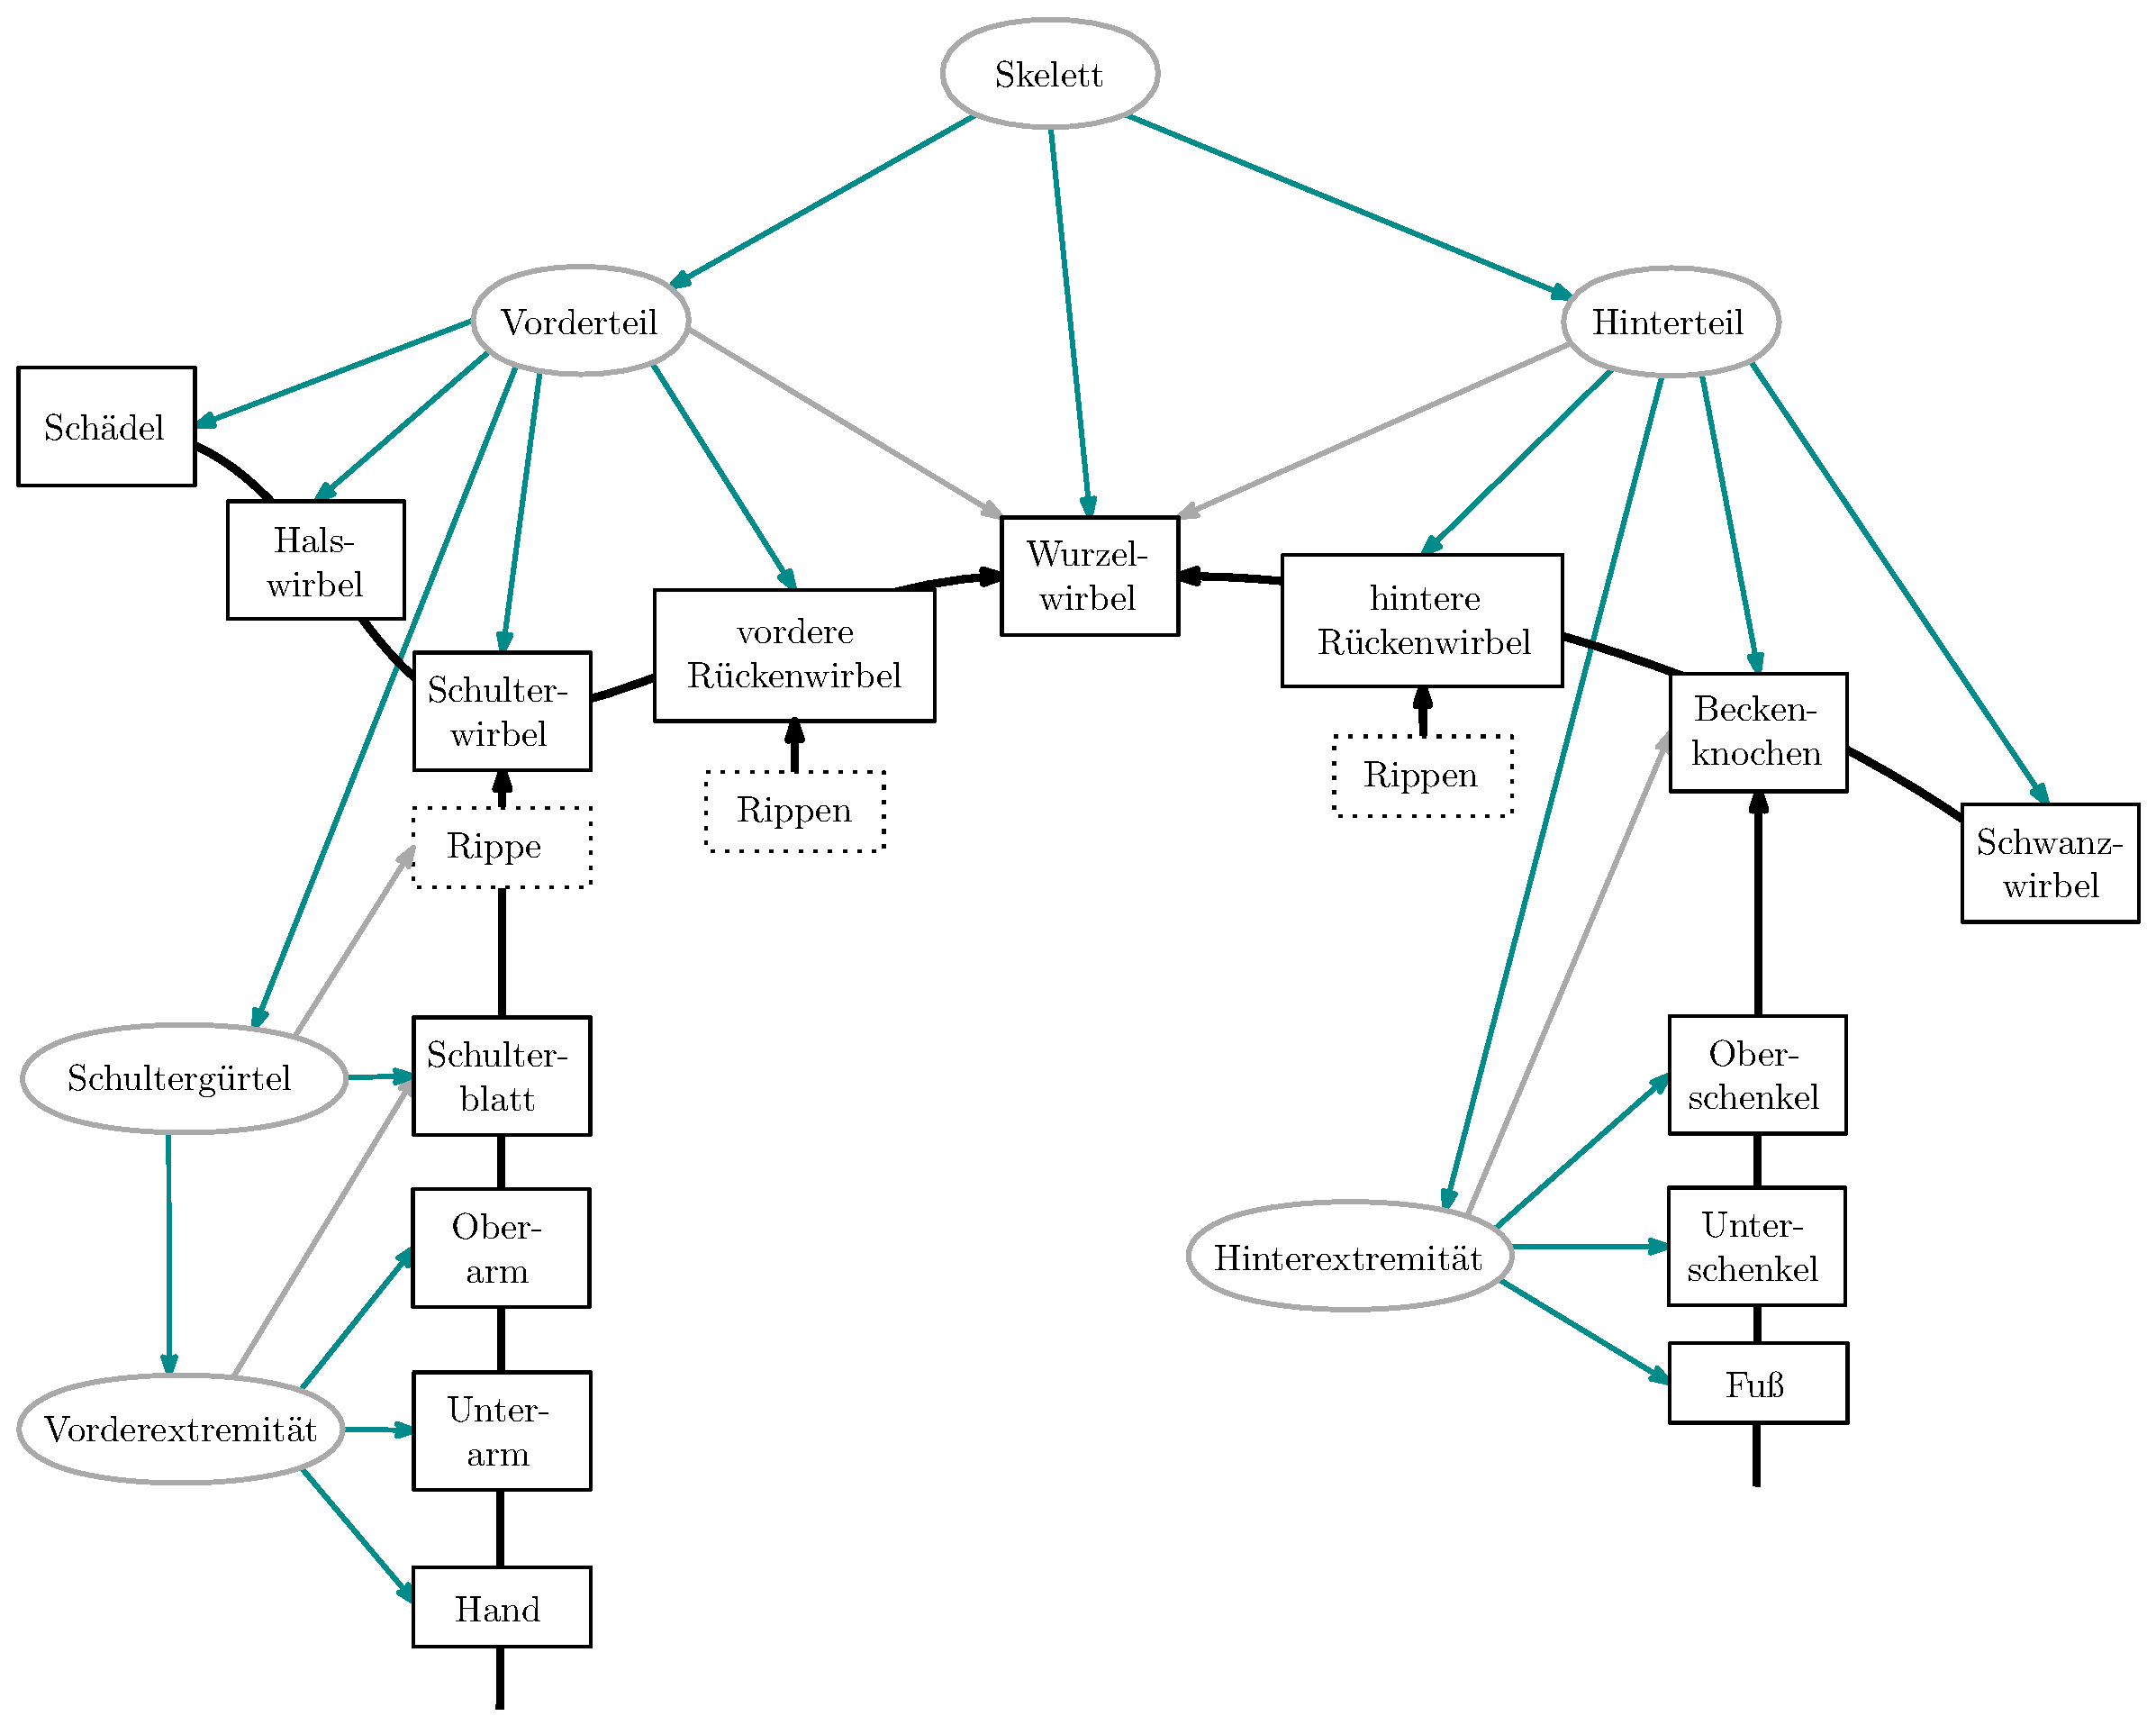
\includegraphics[height=15cm, angle=90, origin=c]{graphics/grammarGraph}
  \caption{Darstellung der Ersetzungsregeln \bzw Produktionen der Grammatik $G$ als Graph. Elliptische Knoten sind Nichtterminalsymbole, rechteckige Knoten Terminalsymbole. Türkisfarbene Kanten zeigen auf diejenigen Symbole, durch die ein Nichtterminal bei Anwendung der entsprechenden Regel ersetzt wird. Graue Pfeile zeigen auf das Elternelement eines nichtterminalen Knotens und schwarze Kurven zeigen für Terminale in welcher Richtung das jeweilige Elternelement liegt.}
  \label{grammar_graph}
 \end{figure}

% optionale Elemente
Außerdem sind, wie in den Produktionen $P$ definiert, manche Teile des Skeletts optional. Gegebenenfalls werden also nichtterminale Knoten nur durch Teilmengen der hier angegebenen Knoten ersetzt. Schulterblatt und Beckenknochen werden beispielsweise nur dann generiert, wenn es auch Extremitäten gibt, die daran ansetzen sollen. Der Schultergürtel ist Kindknoten der Rippe am Schulterwirbel. Existiert diese Rippe jedoch nicht, ist er direkter Kindknoten des Schulterwirbels. Bei allen anderen Knoten gilt: fehlt das Elternelement, so wird dieser Knoten nicht eingefügt.

 
\paragraph{Berechnung der Zusatzbedingungen}

Bevor die Grammatik verwendet wird, müssen die Zusatzbedingungen in den Produktionen spezifiziert werden. Bei Ausdrücken $A^x$ muss $x$ bestimmt werden, also wie oft $A$ vorkommt.
Als Grundlage für diese Entscheidungen dient der vorher, auf Grundlage der PCA, gewählte Punkt $p$ und evtl.\ Benutzereingaben (siehe Überblick \ref{section:overview}).

\begin{itemize}
 \item Wie die Anzahl der Wirbel auf Hals ($w_h$), Schwanz ($w_s$) und Rücken ($w_{rv} + w_{rh}$) bestimmt werden, wird in Abschnitt \ref{section:vertebrae_ribs} erklärt.
 
 \item  Wieviele Rippen ($r$) generiert werden wird zufällig bestimmt (siehe ebenfalls Abschnitt \ref{section:vertebrae_ribs}).
 
 \item Ob überhaupt eine Hals- \bzw Schwanzwirbelsäule generiert wird hängt davon ab, ob dieser Teil der Wirbelsäule in derjenigen Wirbelsäule, die durch $p$ vorgegeben wird, eine Länge größer null hat.
 
 \item \emph{Schultergürtel} und \emph{Beckengürtel} werden generiert wenn das Skelett Vorder- \bzw Hinterextremitäten besitzt. Um das zu bestimmen wird \ua betrachtet welchen Wert der Punkt $p$ im Merkmal \emph{Beine mit Bodenkontakt} und welchen Wert er im Merkmal \emph{Flügel} annimmt. Genaueres dazu ist in Abschnitt \ref{section:extremity_generation} zu finden.
\end{itemize}


%-----------------------------------------------
\section{Extremitäten}
\label{section:extremity_generation}

% was ist schon vorgegeben
Die Bestandteile einer Extremität sind durch den Grundbauplan (Abbildung \ref{bauplan_skelett}) vorgegeben und die Länge der Bestandteile durch die Entsprechenden Merkmale des PCA-Datenpunkts $p$. Die Schwierigkeit besteht nun darin in den entsprechenden Ersetzungsregeln (siehe Abbildung \ref{grammar_graph}) auch die Positionierung vorzunehmen.

\paragraph{Positionierung}
% Allgemeine Schwierigkeit Extremitäten zu positionieren
Das Skelett soll in einer Art Ruheposition dargestellt werden (siehe auch Abschnitt \ref{pose}). Im Allgemeinen ist aber nicht klar wie die Ruheposition einer Extremität aussieht. Das ist schon allein daran zu erkennen, dass auf Darstellungen von Wirbeltierskeletten Flügel manchmal ausgestreckt und manchmal eingefaltet sind. Auch Beine sind meist so angeordnet, dass es aussieht als würde das entsprechende Tier gerade laufen. Dies ist auf Abbildung \ref{klippschliefer_farbig} am Beispiel des Klippschliefers sehr gut zu sehen.

Wie in Kapitel \ref{chapter:pca} zur PCA schon erwähnt, ist es deshalb auch schwer möglich die Ausrichtung der Extremitäten \bzw die Winkel an den Gelenken zu erheben und als zusätzliche Dimension für die PCA mitaufzunehmen.
Die Positionierung der Extremitäten bleibt also ein Problem mit unklaren Anforderungen und vielen Freiheitsgraden.

% Einteilung in Kategorien
Ein erster Schritt an das Problem heranzugehen ist es in kleinere Unterprobleme zu zerteilen.
Extremitäten können anhand ihrer Funktion in vier Kategorien eingeteilt werden:
Flügel, Flossen, Extremitäten mit Bodenkontakt (im Folgenden als Beine bezeichnet), und Extremitäten ohne Bodenkontakt, die weder Flügel noch Flossen sind, (im Folgenden als Arme bezeichnet).

\begin{figure}
 \subfloat[$2$ Beine, $2$ Flügel]{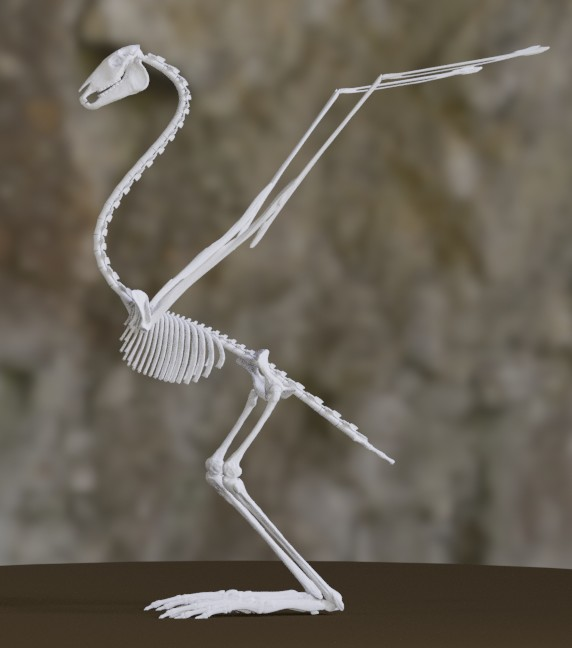
\includegraphics[height=9cm]{../java_skeleton_generation/example_skeletons/bird.jpg}}~
 \subfloat[Känguru, $2$ Beine, $2$ Arme]{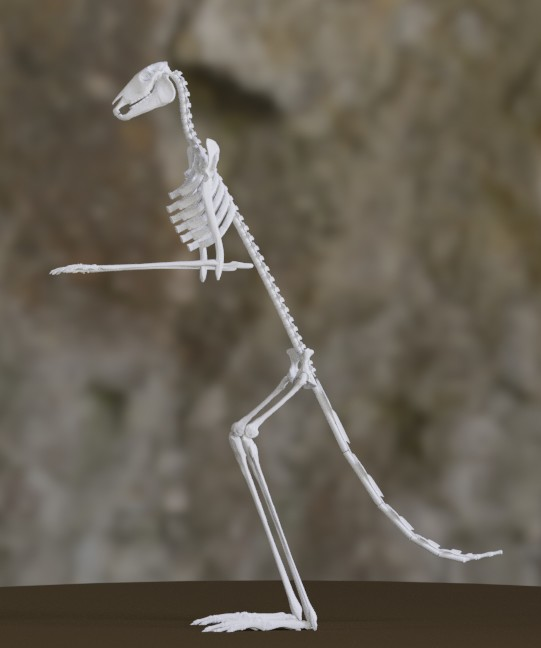
\includegraphics[height=9cm]{../java_skeleton_generation/example_skeletons/kaenguru.jpg}}
 \\
 \begin{center}
  \subfloat[$4$ Flossen]{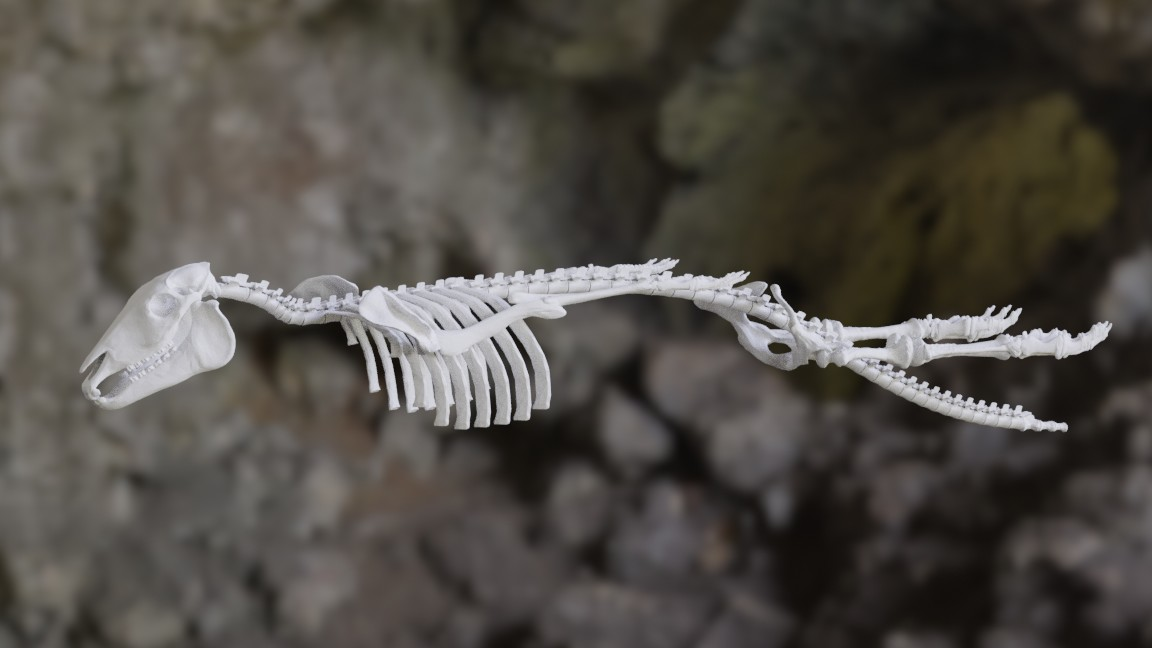
\includegraphics[width=0.8\textwidth]{../java_skeleton_generation/example_skeletons/fish.jpg}}
 \end{center}
 
 \caption{Beispiele generierter Skelette mit verschiedenen Arten von Extremitäten. Die Bedingungen, die verwendet wurden, um die Skelette zu generieren, sind jeweils unter den Bildern zu finden. In (b) wurden die Daten verwendet, die für das Känguru erhoben wurden, mit den zusätzlichen Bedingungen, dass das Skelett $2$ Beine und $2$ Arme haben soll (siehe dazu auch Abschnitt \ref{load_skeletons}). Als Hintergrund wurde \cite{background} verwendet.}
 \label{extremity_orientations}
\end{figure}

Für Flügel, Flossen und Arme gibt es keine besonderen Anforderungen außer, dass sie als solche zu erkennen sein sollten. Deshalb werden sie nach folgenden simplen Anweisungen orientiert (siehe auch Abbildung \ref{extremity_orientations}):
\begin{itemize}
 \item Flossen: Ausrichtung gerade nach hinten (orientiert an Welt-$x$-Achse)
 \item Arme: Der Oberarm zeigt senkrecht nach unten (orientiert an Welt-$y$-Achse), im Ellenbogengelenk ist ein $90^{\circ}$ Winkel und die Hand verlängert den Unterarm nach vorne.
 \item Flügel: Jedes beteiligte Gelenk hat ein Intervall mit festen Grenzen speziell für Flügel, aus dem zufällig ein Winkel gewählt wird.
\end{itemize}

Nun bleibt nur doch die Ausrichtung der Beine, für die die zusätzliche Anforderung gilt, dass sie den Boden berühren sollen.


\paragraph{Bestimmung von Art und Anzahl}

Je nach Art wird die Anzahl der entsprechenden Extremitäten unterschiedlich bestimmt. Als Grundlagen dient der gewählte Punkt $p$ im PCA-Raum. Hier werden die Werte $v_b$ und $v_f$ betrachtet, die $p$, zurücktransformiert ins ursprünglichen Koordinatensystem, für \emph{Beine mit Bodenkontakt} und \emph{Flügel} annimmt. Priorisiert werden die verschiedenen Arten von Extremitäten in der Reihenfolge, wie sie im Folgenden aufgezählt sind.

\begin{itemize}
 \item Beine: Der Wert $v_b$ liegt im Intervall $[0, 2]$ \bzw wenn $v_b < 0$ oder $v_b > 2$, so wird $v_b$ auf $0$ \bzw $2$ festgelegt. Gilt $v_b \in [0, 1]$, so wird mit Wahrscheinlichkeit $v_b$ ein Hinterbein und kein Vorderbein generiert. Gilt $v_b \in [1, 2]$, so wird mit Wahrscheinlichkeit $1$ ein Hinterbein und mit Wahrscheinlichkeit $v_b - 1$ ein Vorderbein generiert.
 
 \item Flügel: Der Wert $v_f$ liegt in $[0, 1]$ \bzw wird, wie bei den Beinen, darauf eingeschränkt. Wenn am Schultergürtel noch keine Extremität festgelegt ist, so wird dort mit Wahrscheinlichkeit $v_f$ ein Flügel generiert.
 
 \item Arme: Die Berechnung basiert auf $v_f$ und funktioniert gleich wie bei den Flügeln.
 
 \item Flossen: Wenn die Gesamtlänge der entsprechenden Extremität klein genug\footnote{Die maximale Länge wurde im Code auf 200px festgelegt. Das ist aber ein beliebig gewählter Wert.} ist, so wird an jedem Extremitätengürtel ohne Extremität eine Flosse generiert.
\end{itemize}

Diese Berechnungen können dazu führen, dass Tiere, wie der Tyrannosaurus Rex, keine Arme bekommen, oder Fische ohne Flossen generiert werden. Das liegt daran, dass weder Arme noch Flossen Eingabemerkmale für die PCA sind. Deshalb verlässt sich der Algorithmus zusätzlich auf Benutzereingaben, die höher priorisiert werden, als die hier angegebenen Berechnungen.

%- - - - - - - - - - - - - - - - - - 
\subsection{Berechnung der Bodenhöhe}
\label{floor_height}

% Warum nicht Höhe 0?
Zunächst könnte man davon ausgehen, dass die Bodenhöhe einfach auf null festgelegt werden sollte. Das Problem hierbei ist aber, dass die von der PCA berechneten Längen für die Extremitäten meist so kurz sind, dass die Beine dann den Boden nicht mehr erreichen würden. Das liegt daran, dass auf den Bildern, die als Eingabebeispiele für die PCA verwendet wurden, der Boden meistens nicht ganz am unteren Rand ist. Hier würde rigoroses Abschneiden der Bilder auf Fußhöhe wahrscheinlich helfen, es würde in vielen Fällen aber auch ein Großteil der Füße verloren gehen.

% Berechnung
Die Höhe des Bodens wird also nachträglich anhand der vorgegebenen Längen der Extremitäten festgelegt.
Theoretisch würde es reichen einfach das kürzeste Bein im komplett ausgestreckten Zustand zu betrachten und den Boden auf die Höhe seines Endpunkts festzulegen.
Das führt aber zu unnatürlich aussehenden Beinen, da das kürzeste Bein dann genau senkrecht nach unten führen muss um den Boden zu erreichen.
Deshalb wird nur ein bestimmter Anteil\footnote{Dieser Anteil ist in der Implementierung mit $0{,}8$ festgelegt, lässt sich aber natürlich auch variieren.} der Länge der Beine betrachtet. So wird erzwungen, dass die Beine, wenn sie auf dem neu definierten Boden stehen, auch etwas gekrümmt sind.

Wie in Kapitel \ref{chapter:biology} beschrieben, gibt es verschiedene Arten von Füßen \bzw Händen. Die oben beschriebene Berechnung geht davon aus, dass der Boden mit der Fußspitze berührt wird. Aber natürlich gibt es auch Wirbeltiere, die mit dem flachen Fuß auf der Erde stehen.
Deshalb wird zusätzlich zur Bodenhöhe noch eine Wahrscheinlichkeit berechnet, dass die Ferse \bzw das Handgelenk den Boden berühren.

Wird die Bodenhöhe nach oben verschoben, weil die Beine insgesamt zu kurz sind, ist diese Wahrscheinlichkeit null.
Sind die Beine so lang, dass schon ohne die Bodenhöhe anzupassen die Ferse \bzw das Handgelenk auf den Boden reicht, so ist sie eins.
Ansonsten ist die Wahrscheinlichkeit 
\[\frac{\text{Beinlänge} - \text{Höhe des Extremitätengürtels über }0}{\text{Länge des Fußes}}\]

Wenn es Vorder- und Hinterbeine gibt, so wird diese Wahrscheinlichkeit für beide berechnet und dann der Mittelwert genommen. Es ist nämlich sinnvoll, dass alle Beine mit dem gleichen Punkt den Boden berühren.


%- - - - - - - - - - - - - - - - - - - - - - - - -
\subsection{Algorithmus zur Ausrichtung der Beine}
\label{leg_algo}

Eine Herangehensweise das Problem der Ausrichtung der Beine zu lösen, wäre inverse Kinematik zu verwenden (siehe Abschnitt \ref{IK}). 
Da das vorliegende Problem aber recht viele Randbedingungen hat, die ausgenutzt werden können, ist es gar nicht unbedingt nötig einen schwergewichtigen Algorithmus zu implementieren, der ein allgemeineres Problem löst.\\
Hier ist \zb in den allermeisten Fällen klar in welche Richtung ein Gelenk gedreht werden muss, um den Fuß dem Boden zu nähern oder ihn vom Boden zu entfernen. Außerdem ist gar kein spezieller Punkt auf dem Boden vorgegeben, der erreicht werden soll.
Deshalb wurde hier ein eigener, recht simpler Algorithmus entwickelt, der auf dieses spezielle Problem angepasst ist.

%Gelenke
Die Gelenke in den Extremitäten werden hier so vereinfacht, dass sie genau einen Freiheitsgrad haben. Eltern- und Kindknochen sind also auf einer gemeinsamen Ebene festgelegt. Die verwendeten Gelenke mit ihren Einschränkungen sind in Abbildung \ref{joints} zu sehen. Der minimale und maximale Winkel für die Gelenke an Schulterblatt und Beckenknochen orientieren sich an der Welt-$y$-Achse, da außerhalb dieses Bereichs keine sinnvollen Ruhepositionen entstehen würden. \\
% Zweiter Freiheitsgrad
Theoretisch haben das Hüft- und das Schultergelenk nicht nur einen, sonder zwei Freiheitsgrade. Sie lassen sich nicht nur nach vorne und hinten bewegen, sondern auch seitlich abspreizen. Das lässt sich auch leicht als zweite Art von Gelenk im Code abbilden. Allerdings liefert dies oft seltsam anmutende breitbeinige Tiere.
Deshalb wurde der zweite Freiheitsgrad hier außen vor gelassen.
Obwohl es natürlich in der Natur auch viele Tiere mit nach außen gestellten Beinen gibt, wie \zb Echsen.
% + max angewinkelte Pos komisch und Drehrichtung ändert sich je nach anderen Winkel


\begin{figure}
  \centering
  \subfloat[Vorderextremität]{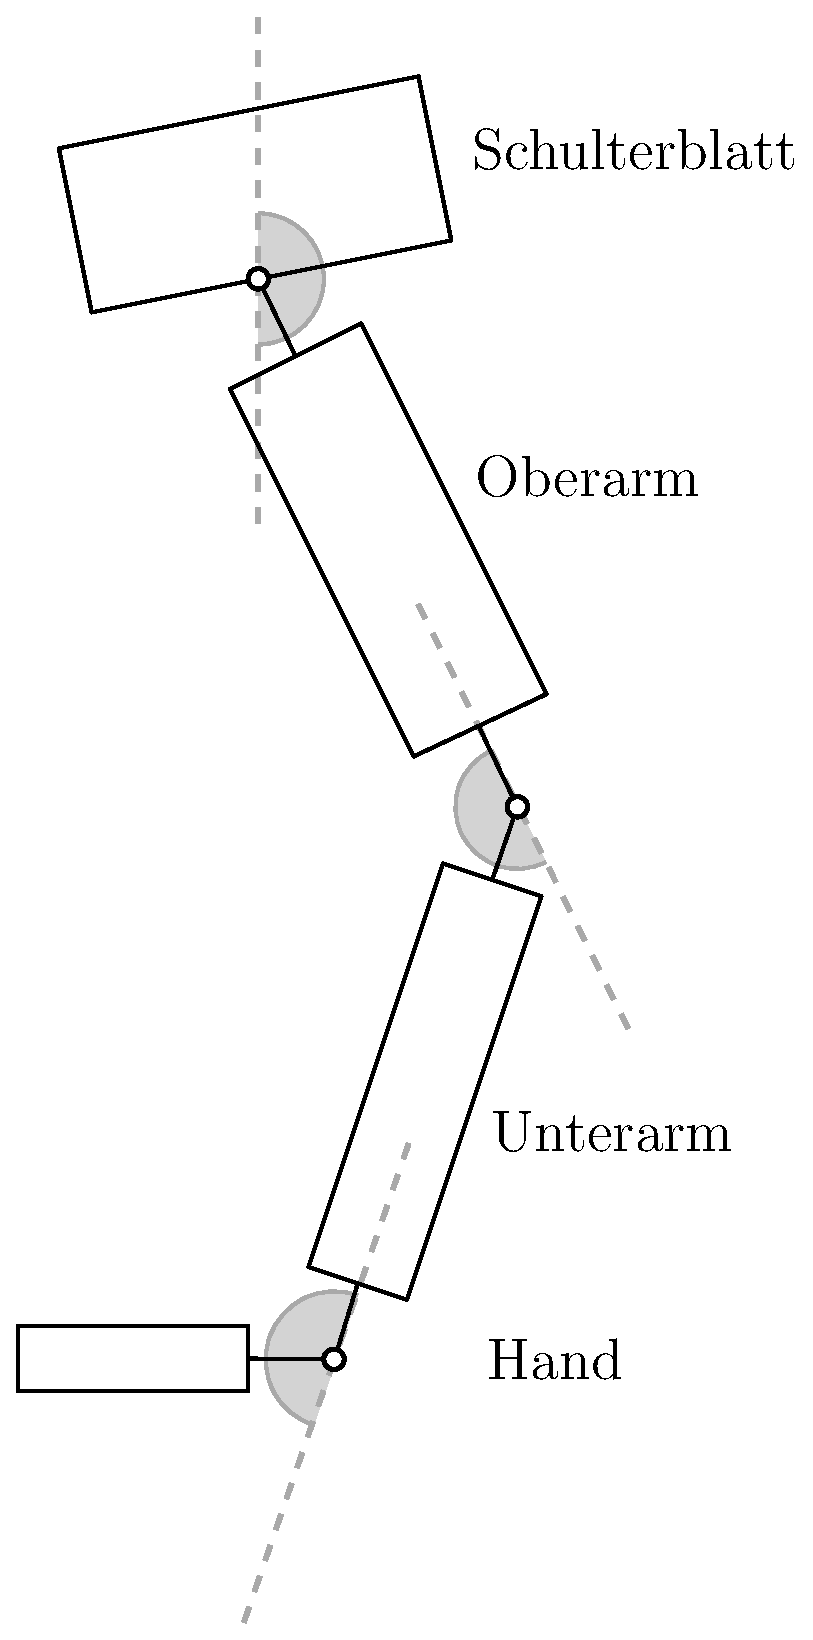
\includegraphics[height=0.3\textheight]{graphics/armJoints}}
  \hspace{3cm}
  \subfloat[Hinterextremität]{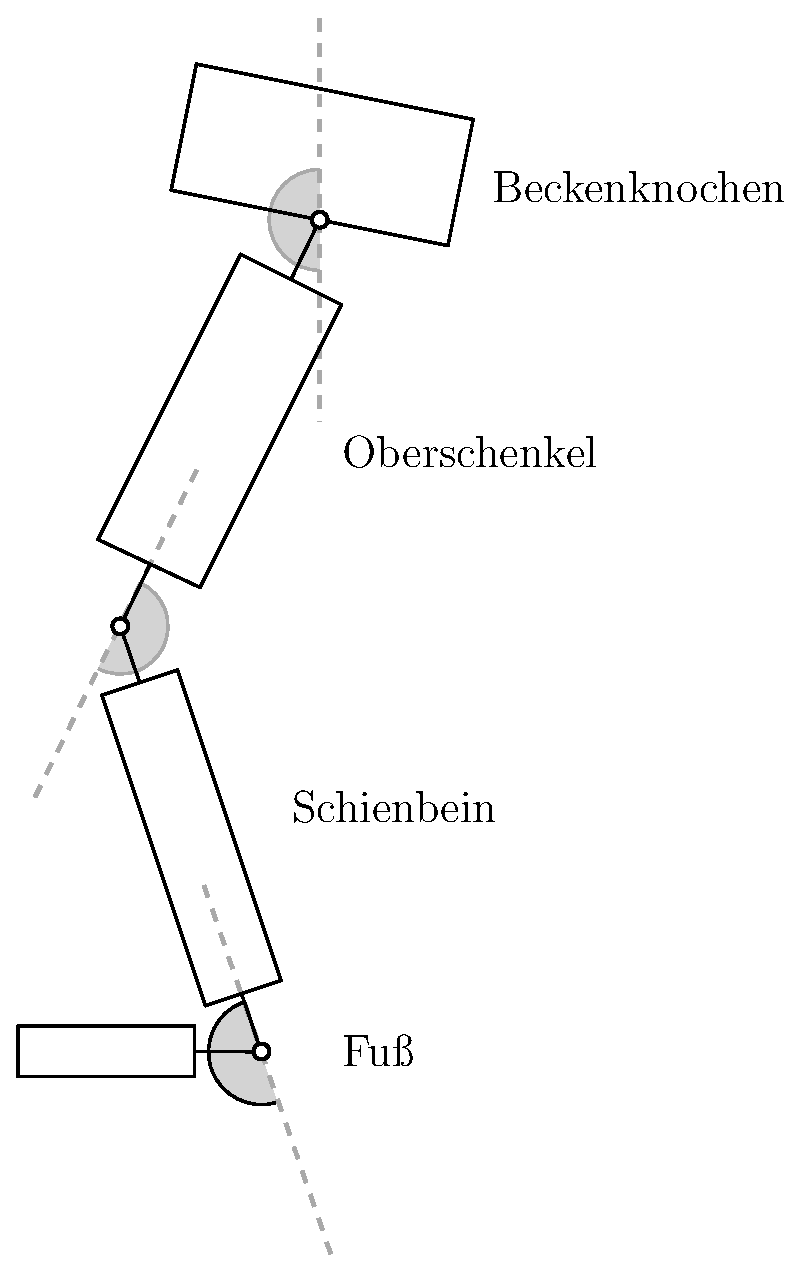
\includegraphics[height=0.3\textheight]{graphics/legJoints}}
  
  \caption{Visualisierung der Bewegungsradien für die Gelenke in Extremitäten mit Bodenkontakt. Darstellung in Seitenansicht (wie in Abbildung \ref{bauplan_skelett}). Die grauen Halbkreise zeigen die möglichen Winkel für eine Ruheposition des Skeletts. Unterarm, Unterschenkel und Fuß können jeweils maximal die Verlängerung des darüberliegenden Knochens bilden und minimal komplett an ihm anliegen. Oberarm und Oberschenkel können nicht über die Senkrechte hinaus gedreht werden.}
  \label{joints}
 \end{figure}

\paragraph{Ablauf}
% iterativ, Drehrichtung
Der Algorithmus geht iterativ vor.
In jedem Schritt wird für jedes Gelenk berechnet ob sein Winkel vergrößert oder verkleinert werden muss, um den dazugehörigen Knochen näher zum Boden zu bewegen.
Mit dem dazugehörigen Knochen ist hier derjenige der beiden an das Gelenk anschließenden Knochen gemeint, der das Kindelement des anderen ist.
Die Drehrichtung lässt sich relativ leicht herausfinden indem die Ausrichtung des Knochens mit der Welt-$y$-Achse verglichen wird. Je senkrechter der Knochen ausgerichtet ist, desto ausgestreckter ist das Bein.
Es gibt also globale Randbedingungen und lokale Einschränkungen je nach Gelenk. % Problematik mit lokalen Winkelkonstraints vs. globalen Berechnungen für Abstand zum Boden?

% Startposition, Bewegungseinschränkungen
In der Startposition ist die Extremität maximal angewinkelt. Die Gelenke beginnen also mit ihren kleinst- \bzw größtmöglichen Winkeln. In den folgenden Iterationen wird dann derjenige Endpunkt der Extremität dem Boden genähert, der zum Schluss Bodenkontakt haben soll. 
Eine andere Möglichkeit wäre mit einer komplett ausgestreckten Extremität zu beginnen und den Fuß von unten der Bodenhöhe anzunähern. Das würde wahrscheinlich genauso gut funktionieren.

Ohne weitere Einschränkungen kann es nun passieren, dass unnatürliche Positionen auftreten, in denen sich \zb der Fußspann näher am Boden befindet als die Fußsohle.
Oder es kann passieren, dass ein Knochen über die positive Welt-$y$-Achse hinaus gedreht wird. Das Problem dabei ist, dass die Einschränkungen an den Gelenken nicht zulassen, dass der Knochen sich unbegrenzt in diese Richtung weiterdreht und der Knochen dann "`feststeckt"'. Deshalb wird nach jeder Drehung festgestellt ob solch eine Situation eingetreten ist und wenn ja, wird die Drehung rückgängig gemacht.
Die Drehung wird ebenfalls rückgängig gemacht, falls sie bewirkt, dass ein Knochen unterhalb der Bodenhöhe liegt.
So ist zu jeder Zeit durch Invarianten garantiert, dass die Knochen auf der "`richtigen"' Seite der $y$-Achse und oberhalb der Bodenhöhe liegen.

% Verkleinerung der Größe der Drehwinkel
In jeder Iteration werden die Winkel, um den die Gelenke gedreht werden, um einen bestimmten Anteil verkleinert. Zu Beginn soll mit großen Veränderungen eine grobe Ausrichtung der Gelenke vorgenommen werden, die dann immer weiter verfeinert wird.
Der Startwinkel darf nicht zu klein sein, weil die Gelenke sonst ihre Zielpositionen nicht erreichen können. Ist der Startwinkel allerdings zu groß, bewirkt das in vielen Fällen, dass in den ersten Schritten des Algorithmus keine Drehung durchgeführt werden kann, weil die oben genannten Randbedingungen durch den großen Winkel verletzt werden.\\
Die Verkleinerung des Winkels darf nicht zu schnell geschehen, weil dann auch die Endposition nicht erreicht werden kann. Wenn sie aber zu langsam geschieht passiert in vielen Schritten wiederum nichts wegen verletzter Randbedingungen.\\
Durch Ausprobieren wurden folgende Zahlen als sinnvoll erachtet: Startwinkel $40^{\circ}$, später dann jeweils $\frac{6}{7}$ davon.

Falls sich der Abstand zum Boden kaum verändert, liegt also die Vermutung nahe, dass die Gradzahl zu groß ist und deshalb alle möglichen Winkeländerungen invalide sind. Deshalb wird in diesem Fall die Gradzahl für die nächste Iteration stärker verkleinert (halbiert).

% Probleme bei sehr kurzen Beinen
Treten sehr kurzen Beinen auf, hat der Algorithmus außerdem einige kleine Probleme. Diese werden genauer in Abschnitt \ref{leg_positioning_short_legs} beschrieben. Da die Beine aber in diesen Fällen, wie gesagt, sehr kurz sind, ist es für den Gesamteindruck gar nicht besonders wichtig wie genau sie angeordnet sind.

\paragraph{Vergleich mit echten Beinstellungen}
% Vergleich echter und generierter Beinstellungen
Wie in Kapitel \ref{chapter:additional_features} beschrieben, lassen sich auch die Eingabebeispiele der PCA laden. Bei ihnen sind dann alle Attribute, die die PCA liefert, schon festgelegt. Alle anderen müssen jedoch noch generiert werden.
Dazu gehören auch die Beine.
Vergleicht man nun die Beinstellung, die der oben beschriebene Algorithmus generiert, mit der Beinstellung auf dem Eingabebild, lassen sich teilweise sehr große Unterschiede feststellen. In Abbildung \ref{extremity_orientations} b wurde ein Känguru generiert. Hier ist die Beinstellung relativ realistsch. Beim Elefanten in Abbildung \ref{elefant} hingegen weicht die Beinstellung stark vom Eingabebild ab.

\begin{figure}
 \subfloat[generiertes Skelett]{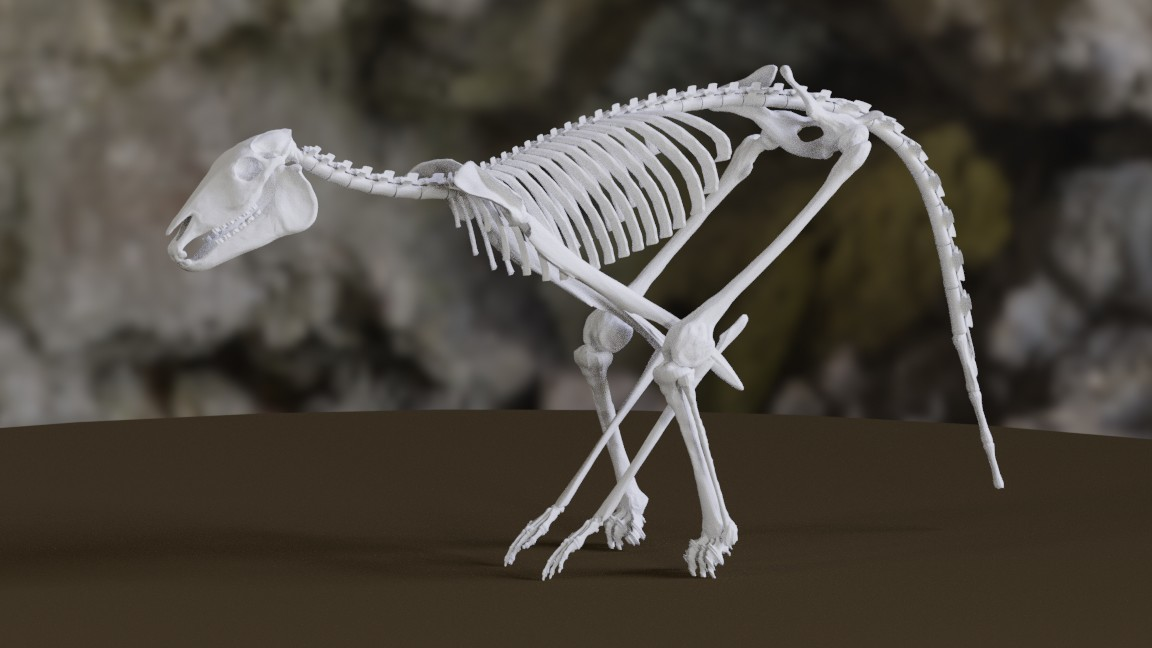
\includegraphics[height=4.5cm]{../java_skeleton_generation/example_skeletons/elefant.jpg}}~
 \subfloat[Eingabebild]{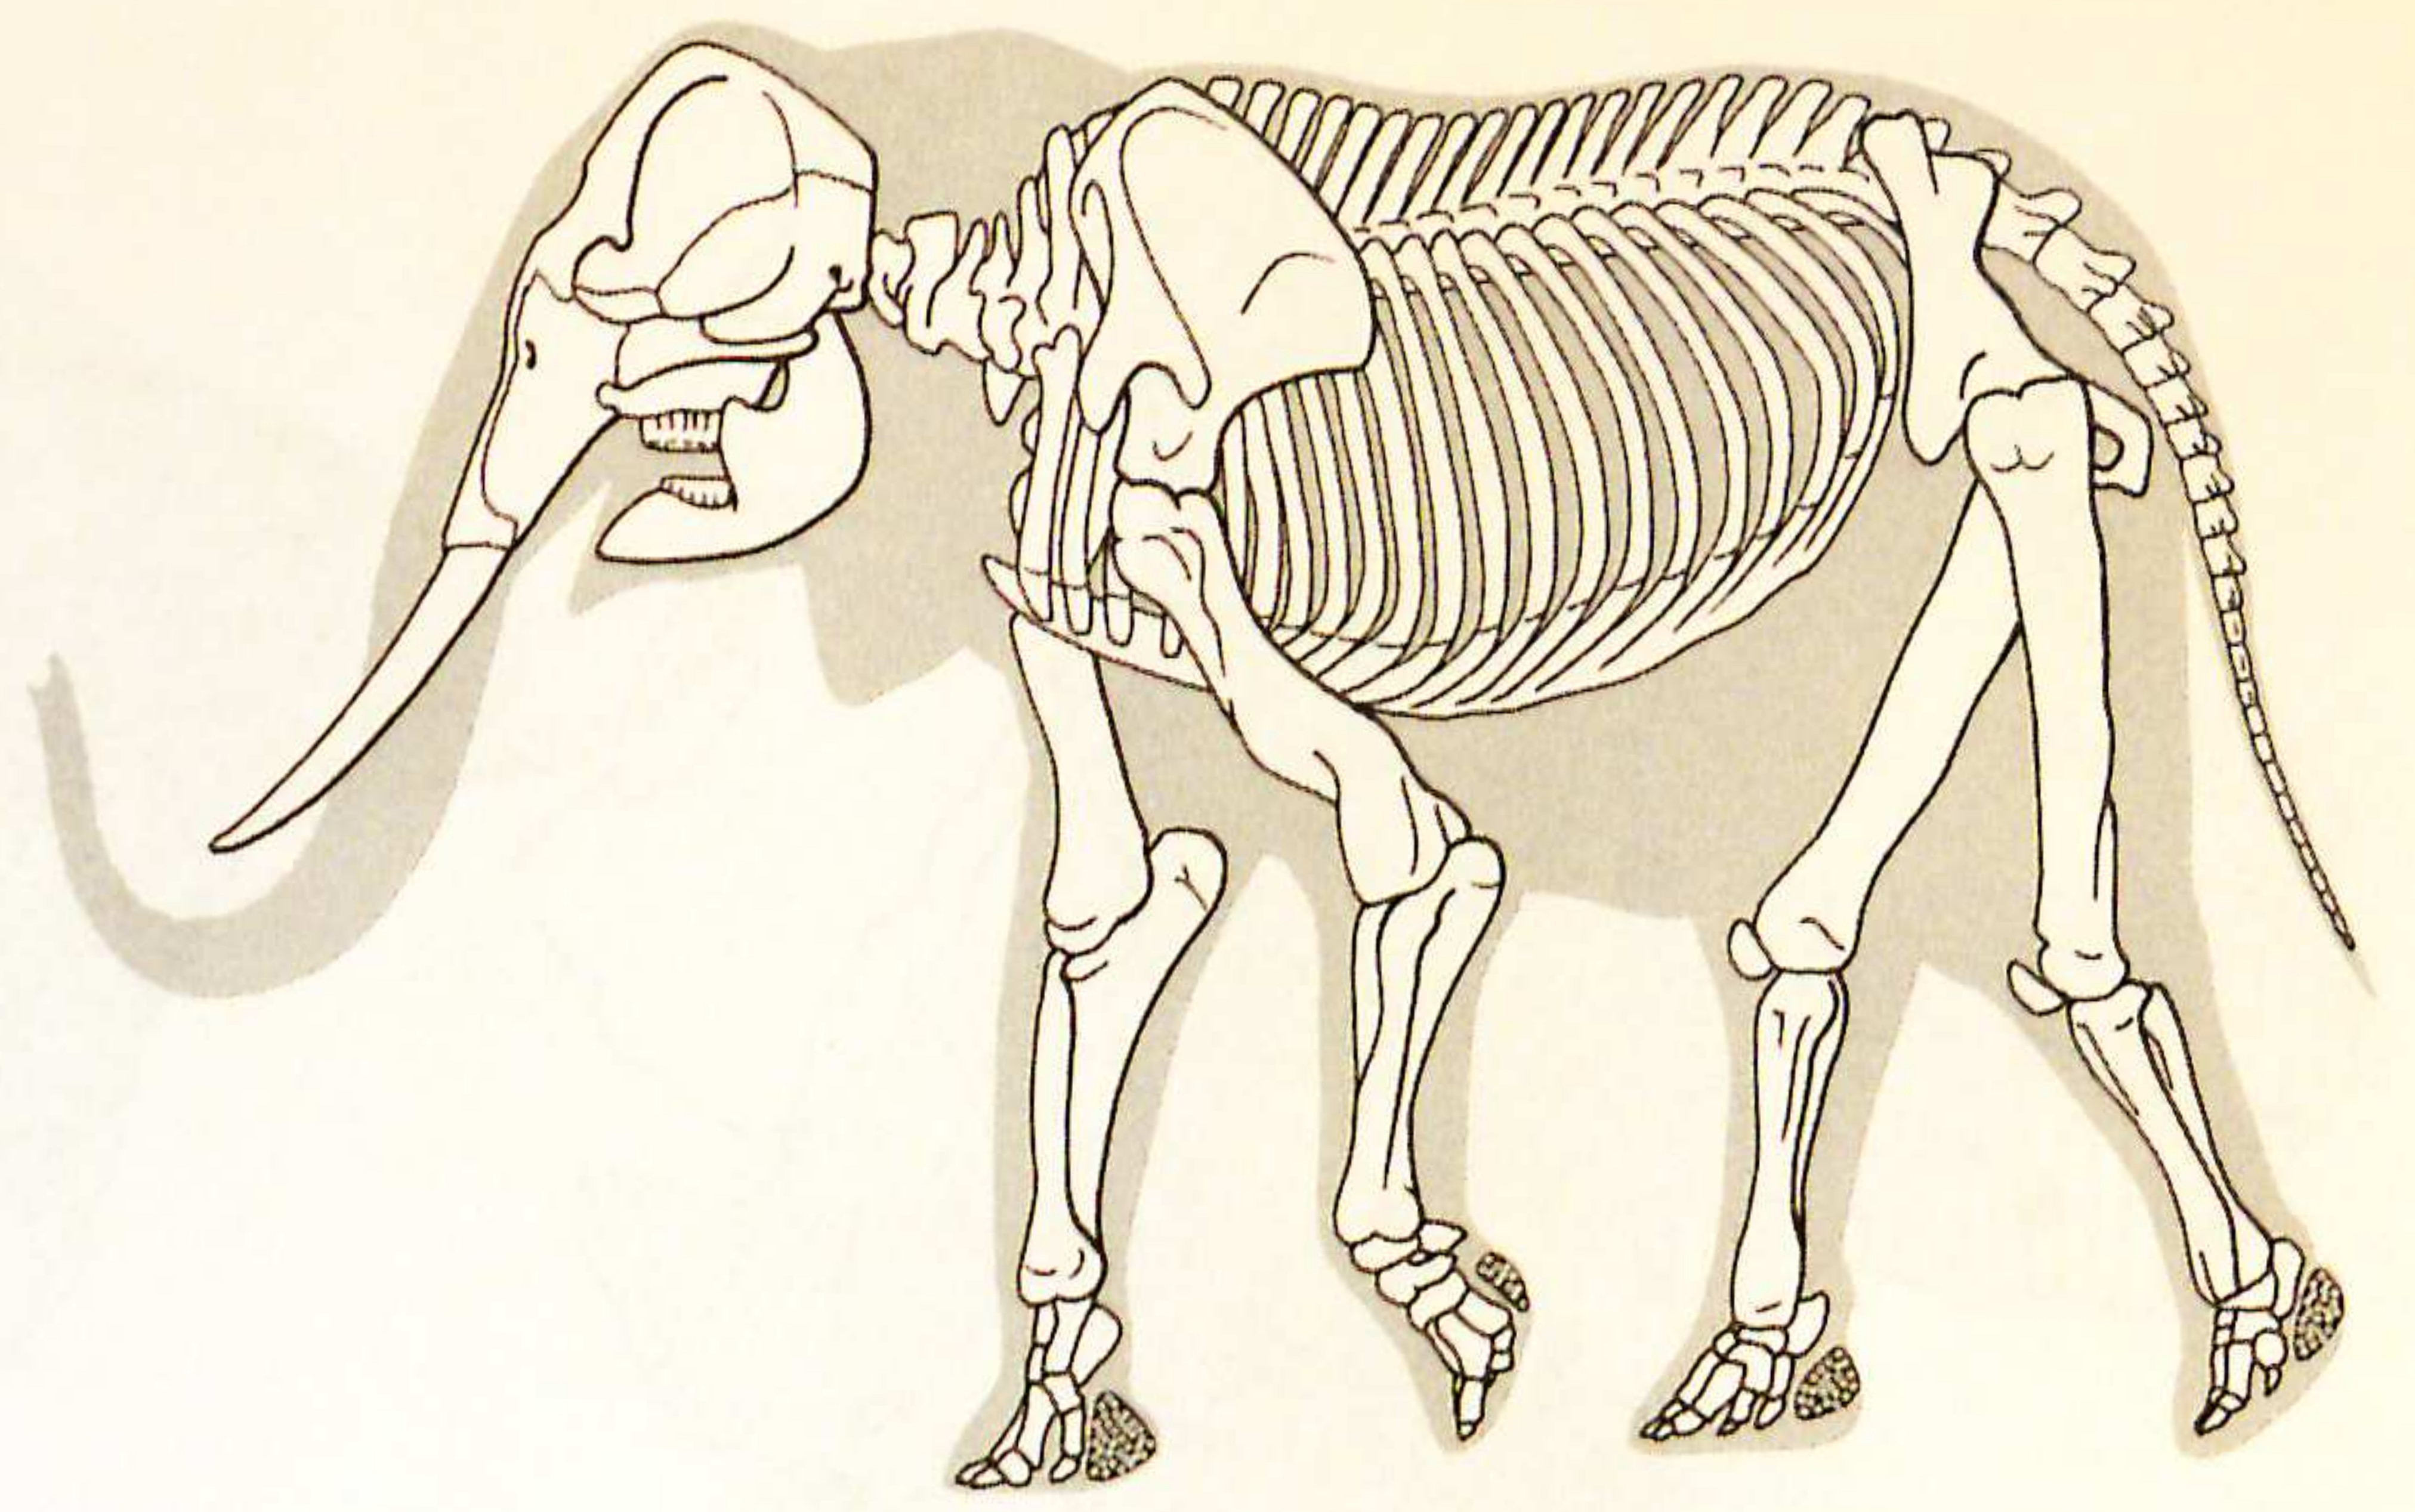
\includegraphics[height=4.5cm]{../PCA/Skelettbilder/Afrikanischer_Elefant.jpg}}
 
 \caption{(a) Skelett eines Elefanten, das anhand der erhobenen Daten generiert wurde. Als Hintergrund wurde \cite{background} verwendet. (b) Die Abbildung des Skeletts eines Elefanten, die auch als Eingabe für die PCA verwendet wurde.}
 \label{elefant}
\end{figure}


% Mehr Infos nötig für Verbesserungen
Um in allen Fällen eine realistisch wirkende Positionierung der Beine zu bekommen, müsste noch sehr viel mehr Arbeit in den Algorithmus gesteckt werden. Außerdem bräuchte der Algorithmus mehr Informationen zum Tier. Solche Zusatzinformationen könnten beispielsweise die Art des Fußes oder die Fortbewegungsart sein. Auch könnte es helfen, wenn es eine sinnvolle Möglichkeit gäbe die Winkel an den Gelenken als Dimension für die PCA mitaufzunehmen. Dafür müsste man sich aber, wie zu Beginn des Kapitels schon erwähnt, auf eine kanonische Ruheposition einigen und dann auch noch Beispiele in genau dieser Position finden.

% für Weiterverwendung werden Beine sowieso angepasst
Ein fertig generiertes Skelett wird höchstwahrscheinlich auch noch weiterverarbeitet. Soll \zb ein animiertes Tier daraus werden, so müssen Bewegungszyklen geschaffen werden. Dafür muss jedes Gelenk vielfach bewegt werden. Soll ein Tier mit Haut und Muskeln daraus werden, so müssen Muskeln an den Knochen ansetzen, die dann einen nicht unerheblichen Anteil an der Positionierung der Beine haben.

% Beinalgo nicht weiter anpassen
Die von dem hier beschriebenen Algorithmus generierte Position kann also gut als erster Eindruck dienen muss aber in den meisten Fällen noch angepasst werden. Ausgehend von der gegebenen Datenlagen und von den zu erwartenden Anwendungen ist es aber nicht sinnvoll den Algorithmus weiter zu verfeinern.

%--------------------------------------
\subsection{Zusätzliche Ansatzpunkte für Extremitäten}

Ansatzpunkte für Extremitäten sind zunächst der Hüftgürtel und der Schultergürtel. Um auch die Generierung fantastischer Tiere (siehe Abschnitt \ref{biology_mythology}) zu ermöglichen, ist es aber möglich dies zu erweitern. Um die Anzahl der zusätzlichen Extremitäten zu bestimmen, ist es am einfachsten sich auf Benutzereingaben zu verlassen. Die Beispieldaten für die PCA sind nur echte Wirbeltierskelette. Deshalb lassen sich aus Punkten im PCA-Raum keine Informationen zu zusätzlichen Extremitäten ableiten.

\paragraph{Zwei Extremitätenpaare pro Extremitätengürtel}
Eine einfache Möglichkeit ist zunächst die Anzahl der möglichen Extremitätenpaare von zwei auf vier zu erhöhen, indem einfach an der Hüfte und der Schulter jeweils zwei Paare ansetzen dürfen. Dafür wurden an der Hüfte \bzw der Schulter mehrere Gelenke direkt hintereinander angelegt. Das ermöglicht beispielsweise Tiere wie den Pegasus (siehe Abbildung \ref{pegasus}).\\
Um das zu ermöglichen, wird die Grammatik $G = (\Sigma, N, S, P, p)$ aus Abschnitt \ref{section:grammar} zu einer Grammatik $G' = (\Sigma', N', S, P', p')$ erweitert, mit $\Sigma' = \Sigma \cup \{\text{Beckenknochen2}\}$ und \mbox{$N' = N \cup \{\text{\emph{Schulterpartie2}}\}$}. Das Terminal "`Beckenknochen2"' steht hier für einen Beckenknochen mit zwei Gelenken für Extremitäten. Die Produktionen in $P$ für \emph{Vorderteil, Schulterpartie} und \emph{Beckengürtel} werden in $P'$ durch folgende Produktionen ersetzt. Außerdem wird eine Produktion für \emph{Schulterpartie2} eingefügt. Die Parameter in $p'$ sind die gleichen wie in $p$, nur dass $e_v$ und $e_h$ (die Anzahl der Vorder- \bzw Hinterextremitäten) in $p'$ auch den Wert $2$ annehmen können.

\begin{align*}
 \text{\emph{Vorderteil}} \rightarrow &\text{ Wirbel}^{(w_{rv} - r)^+}\\
    &\text{ [Wirbel ( Rippe )]}^{(\text{min}(w_{rv}-3, r-3))^+}\\
    &\text{ Wirbel ( \emph{Schulterpartie2} )}^{\vphantom{(}}\\
    &\text{ Wirbel ( Rippe$^{(\text{min}(1, r-1))^+}$ )}\\
    &\text{ Wirbel ( \emph{Schulterpartie} )}^{\vphantom{(}}\\
    &\text{ \emph{Hals}}^{\vphantom{(}}\\
 \text{\emph{Schulterpartie2}} \rightarrow &\text{ Rippe$^{\text{min}(1,r-2)}$ \emph{Schultergürtel}$^{(e_v-1)^+}$}\\
 \text{\emph{Schulterpartie}} \rightarrow &\text{ Rippe$^{\text{min}(1,r)}$ \emph{Schultergürtel}$^{\text{min}(1, e_v)}$}\\   
 \text{\emph{Beckengürtel}} \rightarrow &\text{ [Beckenknochen \emph{Hinterextremität}]$^{\text{min}(1, e_h) \cdot |e_h - 2|}$}\\
    &\text{ [Beckenknochen2 ( \emph{Hinterextremität} ) \emph{Hinterextremität}]$^{(e_h - 1)^+}$}
\end{align*}

Die zweite Schulterpartie beginnt am zweiten Wirbel hinter der ersten Schulterpartie und erzeugt ebenfalls einen Schultergürtel, falls zwei Extrmitäten an der Schulter des Tieres ansetzen sollen. Am Beckengürtel wird anhand der Anzahl der Extremitäten entschieden ob der einfache Beckenknochen oder der "`Beckenknochen2"' mit zwei Gelenken erzeugt werden soll.

% Keine Flügel und Arme an der Hüfte
Flügel und Arme dürfen hierbei nur an der Schulter ansetzen, Beine und Flossen an beiden Stellen. Der Grund dafür ist, dass die meisten generierten Skelette seltsam wirken, wenn an der Hüfte Flügel oder Arme ansetzen und dafür an der Schulter Beine beginnen. Das liegt daran, dass existierende Tiere mit Flügeln oder Armen ihren Schwerpunkt im hinteren Bereich haben und sie auf den Hinterbeinen stehen. Deshalb wird die Wirbelsäule durch die PCA auch dementsprechend angelegt.

\begin{figure}
 \centering
 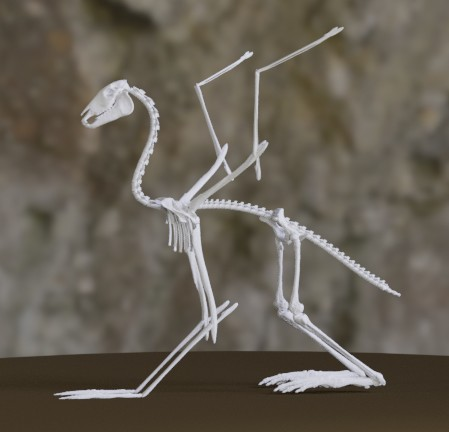
\includegraphics[width=0.6\textwidth]{../java_skeleton_generation/example_skeletons/pegasus.jpg}
 \caption{Beispiel für ein Skelett, dass mit folgenden Bedingungen generiert wurde:\\ $4$ Beine, $2$ Flügel. Mehrere Extremitätenpaare pro Extremitätengürtel waren erlaubt. Als Hintergrund wurde \cite{background} verwendet.}
 \label{pegasus}
\end{figure}


\paragraph{Mehrere Extremitätengürtel entlang der Rückenwirbelsäule}
Eine Überlegung könnte auch sein zwischen Schulter und Hüfte weitere Extremitätengürtel zu erlauben, um \zb Tiere wie den asiatische Drachen erzeugen zu können. \\
Das stellt sich aber als schwierig heraus. Die Wirbelsäule ist zwischen Hüfte und Schulter meist nach oben geschwungen und im Bauchraum befinden sich viele Organe. Ein zusätzlicher Extremitätengürtel würde den Bauchraum einschränken. Außerdem wirkt dann auch die nach oben geschwungene Wirbelsäule anatomisch seltsam.
Verdoppelt man die Schwingung der Wirbelsäule und hängt einfach einen weiteren Rücken hinten oder vorne an, so wirkt es ebenso seltsam, da dann die "`Höcker"' der Wirbelsäule für das Tier wahrscheinlich nicht von Vorteil sind und nur die Fortbewegung erschweren.

Asiatische Drachen sind Spezialfälle, bei denen die zusätzlichen Hüften nicht seltsam wirken, da sie einen langen, schlangenartigen Körper besitzen, bei dem die Wirbelsäule gerade verläuft.

\paragraph{Zweiter Schultergürtel}
Eine weitere Möglichkeit ist Tiere, ähnlich zu Zentauren, zu ermöglichen. Zentauren haben zwei Schultergürtel. Hat das Tier, das generiert wird, einen Hals, der lang genug ist, kann darauf ein weiterer Schultergürtel kurz unterhalb vom Kopf angebracht werden. An diesem Schultergürtel dürfen dann alle Arten von Extremitäten außer Beinen ansetzen. Das wirkt tatsächlich meist auch anatomisch einigermaßen sinnvoll (siehe Abbildung \ref{zentauren}).\\
Hierfür wird die Grammatik $G' = (\Sigma', N, S, P', p')$ aus dem obigen Abschnitt zu einer Grammatik \mbox{$G'' = (\Sigma', N, S, P'', p'')$} mit $p'' = p' \cup \{e_{v2}\}$ erweitert. Der Parameter $e_{v2} \in \{0, 1, 2\}$ steht für die Anzahl der  Vorderextremitäten am zweiten Schultergürtel.
Die Produktion für den \emph{Hals} in $P'$ \bzw $P$ wird in $P''$ durch folgende Produktion ersetzt.

\begin{align*}
 \text{\emph{Hals}} \rightarrow &\text{ Wirbel}^{(w_h - 5)^+}\\
    &\text{ Wirbel ( \emph{Schultergürtel}$^{(e_{v2}-1)^+}$ )}\\
    &\text{ Wirbel}^{\vphantom{(}}\\
    &\text{ Wirbel ( \emph{Schultergürtel}$^{\text{min}(1, e_{v2})}$ )}\\
    &\text{ Wirbel$^2$}\\
    &\text{ Schädel}^{\vphantom{(}}
\end{align*}

Wie an der Schulter, können auf dem Hals, mit dem Abstand von einem Wirbel, zwei Schultergürtel erzeugt werden. Die Gesamtzahl der Wirbel bleibt dabei gleich.  Dies funktioniert auch problemlos, da der Hals, falls vorhanden, immer $\geq 7$ Wirbel besitzt.

Ein solcher Schultergürtel wirkt aber nur sinnvoll, wenn der Hals lang genug ist. Deshalb wird die Benutzereingabe, die einen zweiten Schultergürtel erzwingt in eine Bedingung für die Halslänge umgewandelt und an die PCA weitergegeben (siehe Abschnitt \ref{gui}). Gibt es keine Benutzereingabe, so wird ein zweiter Schultergürtel nur generiert, wenn der Hals lang genug ist.

\begin{figure}
 \subfloat[]{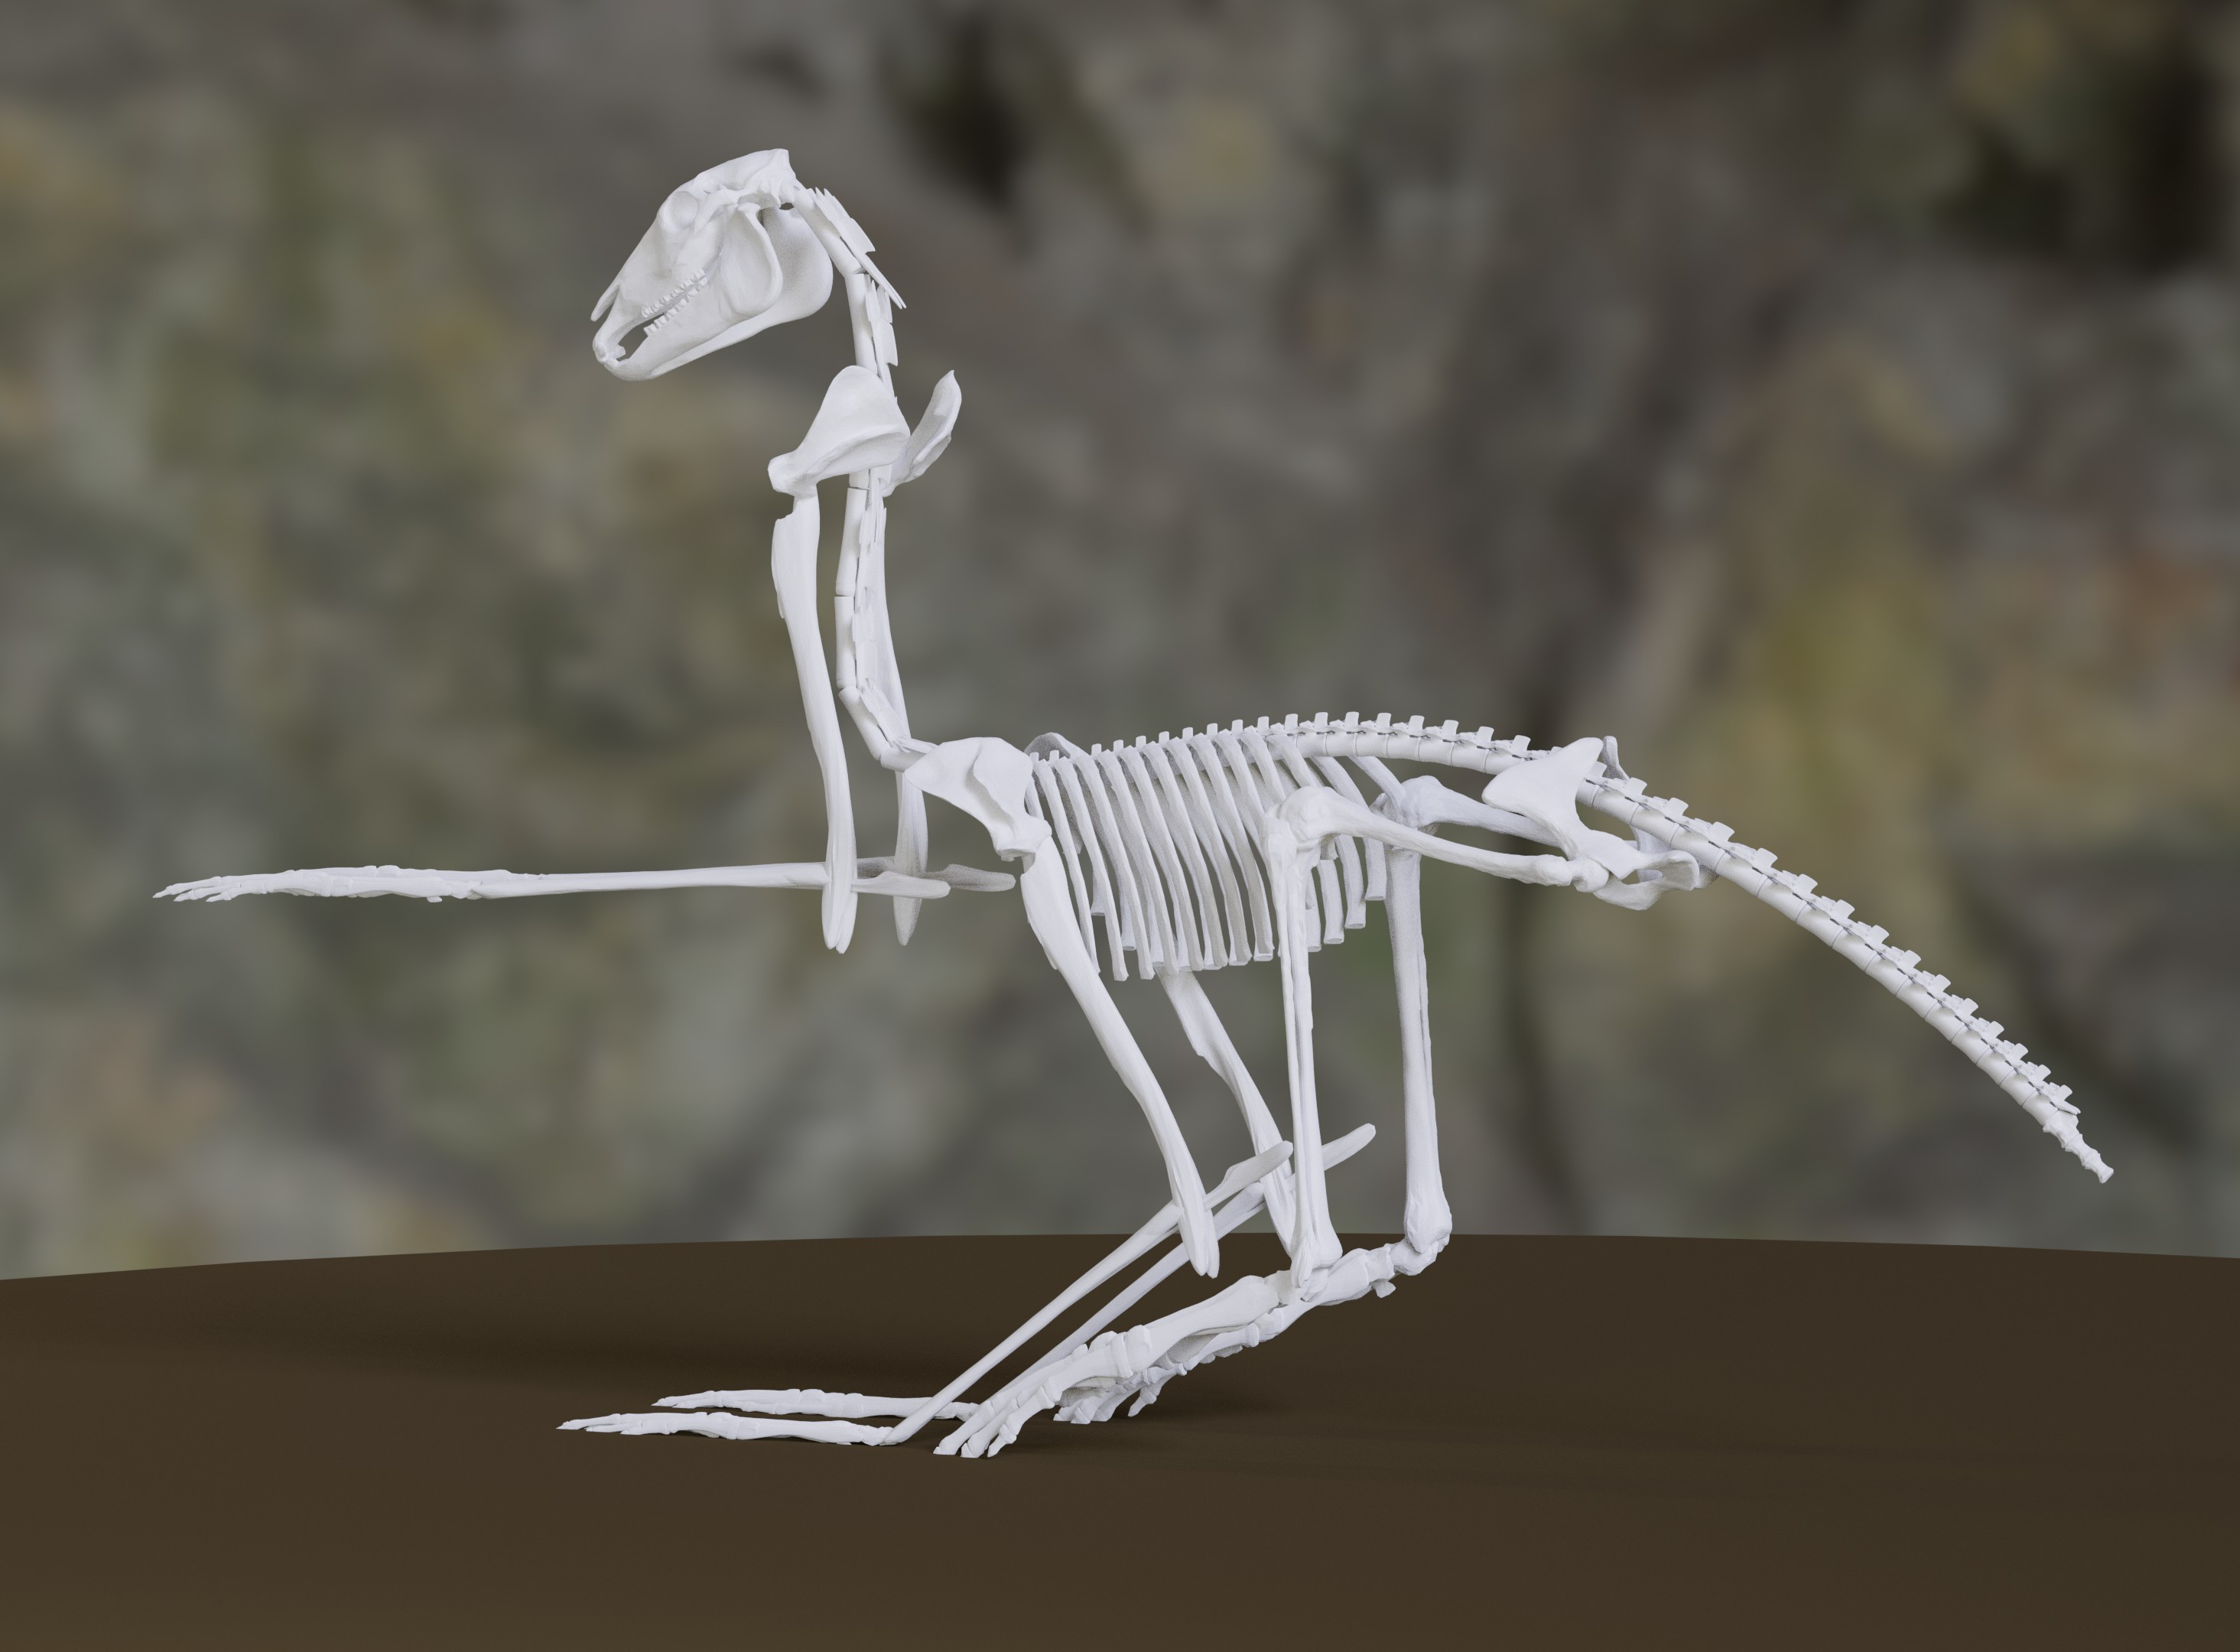
\includegraphics[height=5.5cm]{../java_skeleton_generation/example_skeletons/zentaur1.jpg}}~
 \subfloat[]{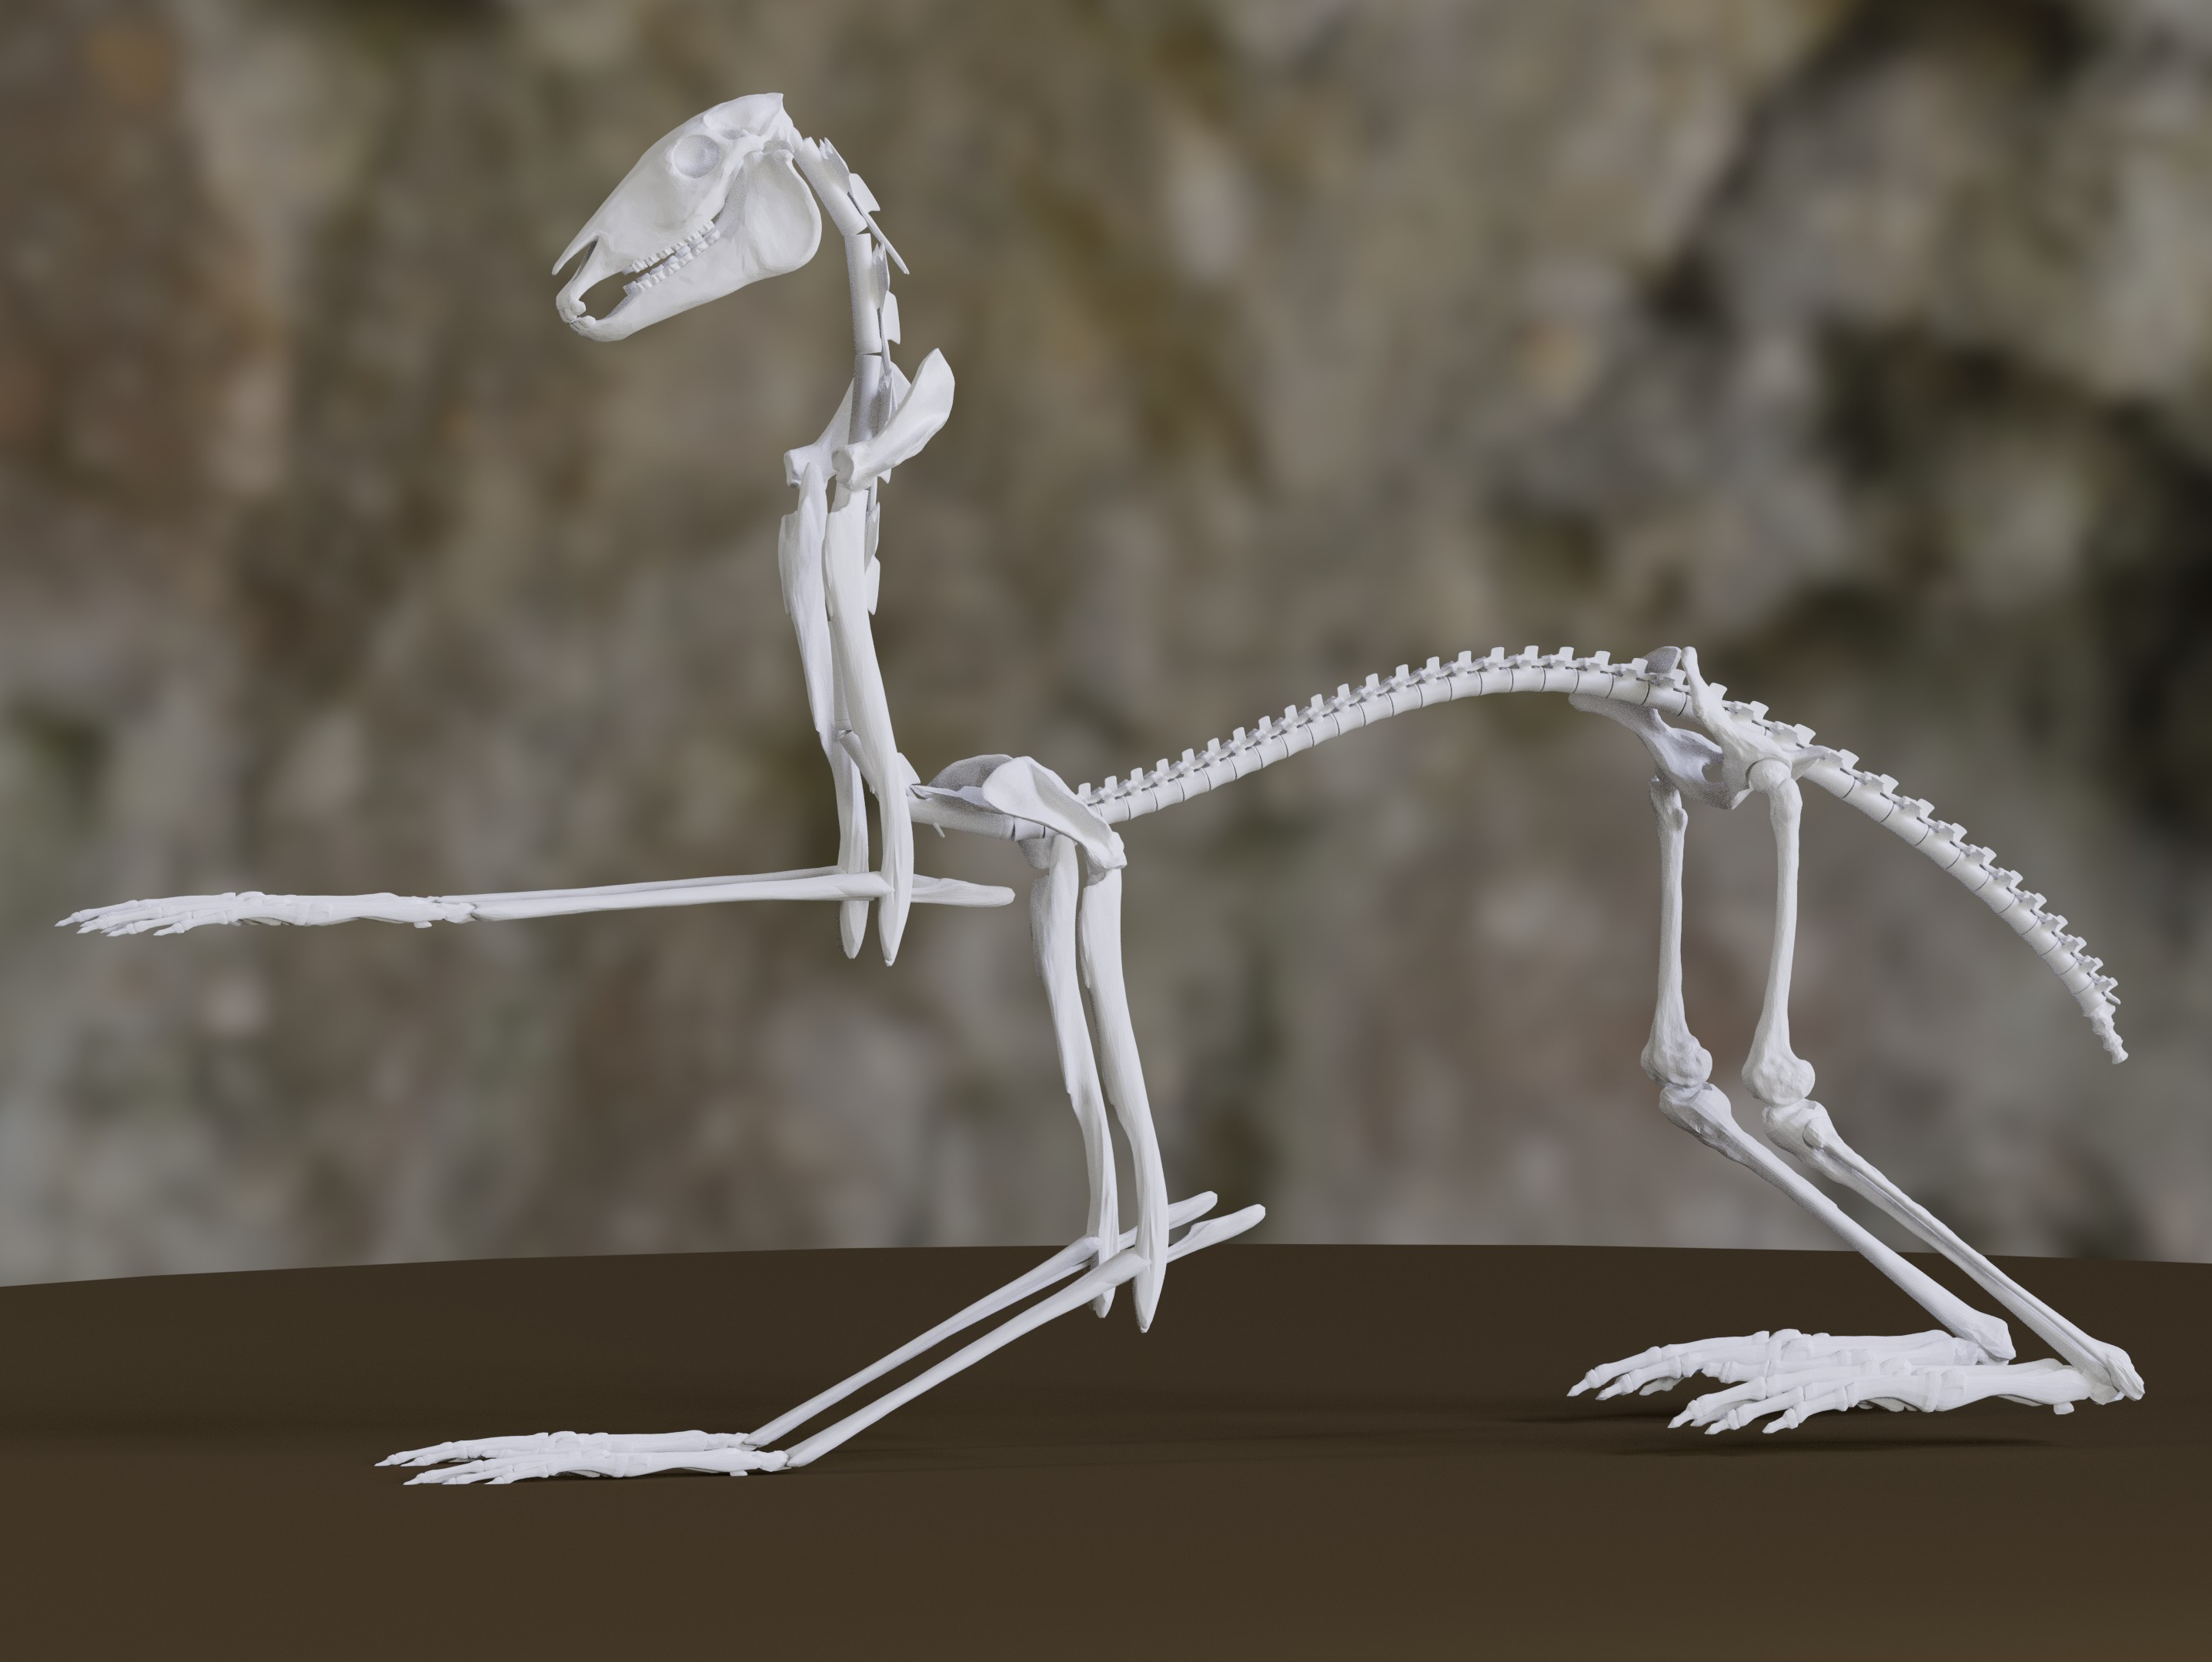
\includegraphics[height=5.5cm]{../java_skeleton_generation/example_skeletons/zentaur2.jpg}}
 
 \caption{Zwei Beispiele für Skelette, die mit folgenden Bedingungen generiert wurden: $4$ Beine, $2$ Arme und ein zusätzlicher Schultergürtel. Mehrere Extremitäten pro Extremitätengürtel sind nicht erlaubt. Als Hintergrund wurde \cite{background} verwendet.}
 \label{zentauren}
\end{figure}


%---------------------------------------------------
\section{Wirbel und Rippen}
\label{section:vertebrae_ribs}

Weitere Dinge, die festgelegt werden müssen, sind die Anzahl der Wirbel auf den einzelnen Teilen der Wirbelsäule und die Anzahl der Rippen.

\paragraph{Wirbel}
Die Anzahl der Wirbel orientiert sich an echten Wirbeltierskeletten (siehe Absatz \ref{biology_skeleton}). Auf dem Hals werden $7$ Wirbel generiert, außer das Tier hat Flügel. Dann wird angenommen, dass ein Vogel generiert wird. Dementsprechend wird die Anzahl dann zufällig zwischen $10$ und $30$ geählt. Auf dem Rücken liegen $25$ Wirbel und auf dem Schwanz $5$ bis $20$.
Da der Wurzelknochen in der Mitte der Rückenwirbelsäule liegt (oder zumindest ungefähr, da Bezierkurve bei $0{,}5$ ausgewertet), wird die Rückenwirbelsäule in zwei Teile geteilt. Es werden $13$ Wirbel auf der vorderen Hälfte und $12$ auf der hinteren generiert.

Eine Bézierkurve ist ein Weg im $\mathbb{R}^2$. Sie ist parametrisiert auf $[0, 1]$ und im Allgemeinen nicht nach Bogenlänge parametrisiert. Das heißt die Geschwindigkeit, mit der die Kurve durchlaufen wird, ist nicht konstant. Wertet man die Kurve also bei $0,5$ aus, wurde nicht notwendigerweise die Hälfte der Strecke zurückgelegt.\\
Für die Generierung von $n$ Wirbeln wurde die Kurve einfach an den Stellen $\frac{i}{n}$ ausgewertet, für $0 \leq i \leq n$. Die Länge des $i$-ten Wirbels ergibt sich dann einfach aus den Abstand zwischen den Stellen $\frac{i-1}{n}$ und $\frac{i}{n}$ auf der Bézierkurve. Durch den oben genannten Effekt variiert dann die Länge der Wirbel über den Kurvenverlauf. Die Wirbel werden auf der Bézierkurve aufgereit und so positioniert, dass sie an den ausgewerteten Stellen aneinander stoßen.

Wird die Bézierkurve $B$ nach Bogenlänge umparametrisieren, so erhält man als neuen Paramter:
\[p(t) = \int_0^t \| B'(s) \| ~\mathrm{d}s. \]
Die umparametrisierte Bézierkurve ist dann $t \mapsto B(p(t))$.

Das obenstehende Integral ist jedoch schwer zu berechnen, da im Allgemeinen keine Stammfunktion des Integranden zur Verfügung steht. Es gibt jedoch numerische Methoden, mit denen das Problem gelöst werden kann. \cite{ArcLengthParametrization}

Betrachtet man echte Wirbeltiere, so sind keine einfachen Regeln für die Länge ihrer Wirbel ersichtlich. Es gibt beispielsweise eine Studie, die die Beschaffenheit der  Wirbel von Mäusen untersucht \cite{MouseVertebrae}. In dieser Studie auf Seite $19$, Abbildung $5$, ist sehr gut zu sehen, dass die Länge der Wirbel allein bei Mäusen im Verlauf der Wirbelsäule sehr stark schwankt.

\paragraph{Rippen}
Die Anzahl der Rippen und auch die Ausdehnung des Brustkorbs variiert zwischen Wirbeltieren sehr stark. Es gibt Tiere, die an jedem Wirbel der Rückenwirbelsäule Rippen haben und es gibt Tiere die haben nur ein paar wenige auf dem vorderen Teil.
Deshalb wird die Anzahl der Wirbel $r$ zufällig aus dem Intervall $ [0, n]$, mit $n =$ Anzahl der Rückenwirbel, bestimmt.
Einige Beispiele mit unterschiedlich vielen Rippen sind auch unter den Beispielbildern für die PCA in Abbildung \ref{all_images} im Anhang zu finden.


%-----------------------
\section{Knochenmodelle}
\label{bone_models}

Um ein 3D-Modell des gesamten Skeletts zu erstellen, wird zunächst jeder terminale Knochen als Quader dargestellt. Diese Quader ergeben sich aus Position, Orientierung und Abmessungen des zugehörigen Knochens. Alle Quader zusammen ergeben ein rudimentäres Modell. Jedoch lassen sie sich auch relativ leicht durch feinere 3D-Modelle der entsprechenden Knochen ersetzen. 

\paragraph{Vorverarbeitung der Knochenmodelle}

Die Knochenmodelle müssen im .obj-Format vorliegen, da auch das resultierende Modell dieses Format hat. Außerdem muss jedes Modell an den Koordinatenachsen ausgerichtet und so verzerrt sein, dass es einen Würfel mit Kantenlänge $1$ in jeder Richtung möglichst gut ausfüllt. So ist es sehr einfach die Längen der Knochen auf das entsprechende 3D-Modell zu übertragen.

Bei dieser Vorgehensweise treten jedoch einige Schwierigkeiten auf. Es ist \zb  relativ schwierig herauszufinden wie man die einzelnen Knochen skalieren muss, sodass sie an den Gelenken gut zusammenpassen und nicht verzerrt aussehen. Im Folgenden sind einige Anpassungen aufgezählt, die die Positionierung vereinfachen.
\begin{itemize}
 \item Kleine Fortsätze, die nicht wirklich zur (optischen) Größe des Knochens beitragen, \zb die Fortsätze der Wirbel, ragen aus dem Würfel heraus. Der Knochen ist somit an manchen Stellen etwas länger als vorgegeben.
 
 \item Kanten, bei denen es wichtig ist, dass sie eine bestimmte Länge haben, sind genau auf die Kantenlänge des Würfels abgestimmt. So können sie leicht auf die richtige Länge skaliert werden. 
 Ein Beispiel dafür ist die Länge der Wirbel entlang der Wirbelsäule. Die Wirbel müssen genau aneinander ansetzen. Mit dieser Skalierung lässt sich einfach die Länge des Wirbels auf das Modell übertragen.\\
 Es kann aber auch um Längen gehen, die nur einen Teil des Knochens betreffen.
 Rippen müssen \zb mit ihrer Breite in $x$-Richtung zur Breite des Wirbels passen, an welchem sie ansetzen. Deshalb ist das 3D-Modell der Rippe so skaliert, dass die Kantenlänge des Würfels in $x$-Richtung genau auf die Breite des Wirbels skaliert werden kann und die resultierende Breite der Rippe dann genau dazu passt.\\
 Da die Rippe stark gebogen ist, führt das dazu, dass die Gesamtlänge der Rippe in $x$-Richtung viel länger ist als die Kantenlänge des Würfels. Das Problem daran ist, dass die gegebenen Abmessungen des Knochens dann nicht mehr viel mit der Ausdehnung des eingesetzten 3D-Modells haben. Je nach dem um welchen Knochen es sich handelt, möchte man diesen Effekt evtl.\ vermeiden.
 
 \item Kantenlängen, die nicht speziell vorgegeben werden, \zb die Dicke der Extermiätenknochen, sind einfacher passend zu bestimmen, wenn sie nicht komplett unabhängig von den anderen Raumrichtungen sind. Ist \zb die $x$- und $y$-Skalierung eines Knochens vorgegeben, und die Skalierung in $z$-Richtung soll nur möglichst gut dazu passen, so ist es sinnvoll das 3D-Modell schon so zu speichern, dass die $z$-Richtung relativ zu einer anderen Richtungen angegeben werden kann. Tut man dies nicht, so führt das leicht dazu, dass die Knochen verzerrt aussehen.
\end{itemize}


\paragraph{Offsets zwischen Knochen}
% Gelenke korrekt ausrichten
Es ist eventuell nicht ganz leicht zu erkennen wie die Knochen ineinander greifen \bzw wie die Gelenke die Ausrichtung der Knochen beeinflussen. Das erfordert etwas Wissen zur Anatomie und viel "`Finetuning"'. 

Für jeden Knochen sind für diese Ausrichtung zwei Offsets gespeichert: das Offset zu dem Gelenk, das ihn mit seinem Elternknochen verbindet und das Offset zu dem Gelenk, das ihn mit seinem Kindknochen verbindet (oder mehrere, falls vorhanden). Dies sorgt dafür, dass die Positionierung der Knochen stimmt, egal wie groß sie sind. Ist ein Knochen sehr groß und ein anschließender sehr klein (oder anders herum), so kommt es natürlich trotzdem vor, dass die Gelenke nicht wirklich ineinander passen. Für solche Situationen bräuchte man verschiedene 3D-Modelle, die je nach Gegebenheit eingesetzt werden.

Es wurden vor allem Modelle von Pferde- und Menschenknochen verwendet, da sie leicht verfügbar waren. Manche Knochen sind jedoch auch von anderen Tieren oder keinem speziellen Tier zugeordnet. Das führt \zb bei dem verwendeten Unterarmknochen vom Pferd dazu, dass er etwas überdimensionierte Fortsätze am Ellenbogen bekommen, wenn man ihn stark verlängert. Das liegt daran, dass dieser Knochen beim Pferd eigentlich relativ kurz ist. Ansonsten passen die Knochen verschiedener Wirbeltiere aber erstaunlich gut ineinander.

Leider unterscheiden sich die Knochen verschiedener Tiere dennoch so stark, dass die Offsets für jedes Knochenmodell individuell bestimmt werden müssen. Dies, und die oben genannten Abweichungen von einem Würfel mit Kantenlänge $1$, führt dazu, dass die 3D-Modelle nicht einfach austauschbar sind.
Um andere 3D-Modelle für Knochen zu verwenden, müsste nicht nur das Modell ausgetauscht werden, sondern eben auch die Offsets angepasst werden. Das ist momentan im Programm nicht möglich ohne den Code zu ändern. Dies ließe sich aber leicht hinzufügen. Die Offsets könnten \zb in einer Textdatei gespeichert werden und zusammen mit den Modellen eingelesen werden. 


\paragraph{Spezielle Knochen}

Für die meisten Knochentypen wird genau ein 3D-Modell verwendet. Bei manchen Knochen und in manchen Fällen wirkt das recht seltsam. Man möchte eigentlich etwas mehr Variation haben.

% Köpfe
% Köpfe sind kompliziert $\rightarrow$ Auswahl an Köpfen bereitstellen (evtl. leicht skalier-/verformbar oder ineinander überführbar)
Besonders stark ist dies am \emph{Schädelknochen} zu beobachten. Er variiert, im Gegensatz zu anderen Knochen, bei Wirbeltieren sehr stark. Hier ist es also ein großer Mehrwert verschiedene Modelle anzubieten. Die Frage ist dann nur wie entschieden wird welcher Schädelknochen wann verwendet wird. Eine Möglichkeit wäre in die Grammatik spezifischere Terminalsymbole für verschiedene Schädel und dazugehörige Regeln einzufügen. Tut man dies nicht, gibt es wenig Anhaltspunkte. Es ist deshalb sinnvoll die Auswahl des passenden Schädelknochens dem Nutzer zu überlassen.\\
Bezüglich der Offsets ist der Schädelknochen ein recht einfacher Fall. Die verschiedenen Modelle lassen sich leicht alle gleich skalieren, sodass keine verschiedenen Offsets gespeichert werden müssen.

% Hände und Füße
Bei \emph{Händen und Füßen} ist das Problem ebenso, dass es sehr viele verschiedene Ausprägungen davon gibt (siehe \zb Abbildung \ref{extremities}). Diese lassen sich jedoch gut nach Extremitätentyp unterscheiden, wobei diese Unterscheidung natürlich beliebig fein sein kann. 
Hier wurde die Unterscheidung verwendet, die auch bei der Positionierung der Extremitäten zum Einsatz kommt (siehe Abschnitt \ref{section:extremity_generation}). \\
Es gibt also Flügel, Arme, Flossen und Beine mit Bodenkontakt. Wobei bei Beinen mit Bodenkontakt zusätzlich noch nach dem Winkel unterschieden wird mit dem der Fuß auf den Boden aufkommt. Bei weniger als $45^\circ$ wird eine menschliche Hand eingesetzt, sonst ein Pferdehuf. Arme bekommen ebenfalls eine Hand. Für Flossen wurde kein spezielles Modell eingefügt, bei ihnen wird ebenfalls eine Hand eingesetzt. Flügel haben ein eigenes Modell. In Ermangelung gemeinfreier Modelle fehlen hier aber leider einzelne Bestandteile.

% (Schwanz)Wirbel
Es wurde ein Modell für alle \emph{Wirbel} verwendet. Bei Wirbeltieren gibt es aber sehr viele unterschiedliche Wirbel, die auch in ihrer größe stark variieren. Ein Beispiel ist das Ende der Schwanzwirbelsäule. Hier werden die Wirbel bei echten Tieren kleiner.
Um das Gesamtmodell realistischer zu machen, lassen sich die Modelle der Wirbel verfeinern. Als Beispiel wurde ein zusätzliches Modell eingeführt, dass die letzten drei Schwanzwirbel ersetzt. Es besteht aus drei aufeinanderfolgenden Wirbeln, die zum Ende hin kleiner werden. Das sieht in den meisten Fällen auch gut aus. Ein Nachteil davon ein einzelnes Modell mit drei Wirbeln zu haben ist aber, dass die Positionierung dann nicht mehr so fein erfolgen kann. Anfangs- und Endpunkt des Modells werden auf der Bézierkurve positioniert. Aber die Anfangs- und Enpunkte der einzelnen Wirbel können teilweise stark vom Verlauf der Kurve abweichen.
Dies lässt sich natürlich leicht durch eine weitere Verfeinerung der Modelle beheben, indem jeder der drei Wirbel ein eigenes Modell bekommt.

\newpage
% mehrere Extremitäten an einer Hüfte
Setzten \emph{mehrere Extremitäten} an einer Hüfte an, so ist ein realistisches Modell des Beckenknochens nicht mehr ausreichend, da nicht genug Gelenke vorhanden sind. Dieses Problem wurde so behoben, dass für das Terminal "`Beckenknochen2"' ein kombiniertes 3D-Modell aus zwei einzelnen Beckenknochen erstellt wurde, an dem nun zwei Gelenke vorhanden sind.




